\part{神经系统细胞的细胞生物学和分子生物学}
%\chapter*{神经系统细胞的细胞生物学和分子生物学}
\markboth{神经系统细胞的细胞生物学和分子生物学}{神经系统细胞的细胞生物学和分子生物学}

\begin{figure}[htbp]
	\centering
	\includegraphics[width=0.9\linewidth]{chap07/fig_7_0}
	\caption{嗜热微生物古甲烷杆菌的\textit{线粒体已糖激酶}~\ce{Ca^2+}调节 \ce{K+}通道的晶体结构。
		这是从处于~\ce{Ca^2+}结合开放状态的通道的细胞外侧观察的。
		\textit{线粒体已糖激酶}由 2 个主要的功能结构域组成。
		一种完整的膜蛋白形成 1 个水性孔(蓝色),它选择并传导~\ce{K+},并具有一个在打开和关闭构象之间切换的门;
		细胞内~\ce{Ca^2+}结合门控环(灰色)控制该门。
		当它结合~\ce{Ca^2+}时,所产生的构象变化被机械地传递到孔中,导致其切换到开放状态。}
	\label{fig:7_0}
\end{figure}





在所有的生物系统中(从最原始到最先进),基本的组成部分都是细胞。
细胞通常被组织成在复杂的生物系统中重复的功能模块。
脊椎动物的大脑是模块化系统中最复杂的例子。
复杂的生物系统还有另一个基本特征:
它们是构造性的,也就是说,它们的解剖结构、精细结构和动态特性都反映了特定的生理功能。
因此,大脑的结构及其组成细胞的细胞生物学、生物物理学和生物化学反映了其基本功能,即调节行为。


神经系统由神经胶质细胞和神经细胞组成。
早期将神经胶质细胞视为纯粹的结构元件的观点已经被我们目前的理解所取代,即有几种类型的神经胶质细胞,每种都专门调节神经元功能的一个或多个特定方面。
不同种类的神经胶质细胞在促进和引导神经发育、隔离轴突过程、控制细胞外环境、支持突触传递、促进学习和记忆以及调节神经系统内的病理过程方面发挥着重要作用。
一些神经胶质细胞具有神经递质受体和电压门控离子通道,使它们能够相互通信,并与神经元通信,以支持神经元信号传导。


与神经胶质细胞相比,神经细胞的巨大多样性是神经系统模块的基本单元,这些神经细胞的多样性是基于一个基本细胞规划的变体。
该规划的 4 个特点使神经细胞具有独特的能力,能够在长距离内精确快速地相互交流。
首先,神经元是极化的,一端有感受性树突,另一端有与突触前终末相连的轴突。
这种函数性质的极化将电压脉冲的主要流动限制在一个方向上。
其次,神经元具有电兴奋性。
它的细胞膜含有专门的蛋白质,即离子通道和受体,他们允许特定无机离子的流入和流出,从而产生跨膜电流,形成跨膜电压信号。
第三,神经元含有蛋白质和细胞器,赋予其特殊的分泌特性,使其能够在突触处释放神经递质。
第四,这种在细胞体及其末端之间长距离快速信号传导的系统是由细胞骨架结构实现的,该结构在较慢的时间尺度上介导各种蛋白质、信使核糖核酸和细胞器在 2 个\textit{区室}之间的有效转运。


在本书的这一部分,我们将关注独特的细胞生物学特性,这些特性使神经元和胶质细胞能够实现其各种特殊功能。
重点将放在离子通道的特性上,离子通道赋予神经元以动作电位的形式产生和传播电信号的能力。
在讨论神经元之前,我们首先考虑离子通道共有的一些一般性质,包括选择和传导离子的能力,以及在开放和关闭构象之间进行调控的能力。
神经元使用四大类通道进行信号传导:
(1)静息通道产生静息电位,并成为神经元被动电特性的基础,这些特性决定了突触电位的时间进程、沿树突的分布以及触发动作电位的阈值;
(2) 感觉受体通道对某些感觉刺激作出反应,产生局部受体电位;
(3) 配体门控通道对神经递质作出反应而开放,产生局部突触电位;
以及(4)电压门控通道产生电流,从而产生自传播动作电位。
在这一部分中,我们主要关注静息和电压门控通道。
在第三部分中,我们更详细地考虑了配体门控通道,以及控制其活性的神经递质和第二信使。
感官刺激激活的通道将在第四部分中进行检查。




\chapter{神经系统的细胞} \label{chap:chap7}

神经系统的细胞(神经元和胶质细胞)与一般细胞有许多相似之处。
然而,神经元具有特殊的天赋,能够与体内远处的其他细胞进行精确、快速的通信。
2 个特征赋予了神经元这种能力。


首先,它们具有高度的形态和功能不对称性:
神经元的一端有\textit{接受}树突,另一端有\textit{传递}轴突。
这种排列是单向神经元信号传导的结构基础。


其次,神经元既可\textit{电兴奋}又可\textit{化学兴奋}。
神经元的细胞膜包含特殊的蛋白质(离子通道和受体),它们能够促进特定无机离子的流动,从而重新分配电荷并产生改变跨细胞膜电压的电流。
这些电荷的变化会沿着轴突以动作电位的形式产生去极化波,这是信号在神经元内传播的通常方式。
胶质细胞不太容易兴奋,但它们的膜含有促进离子摄取的转运蛋白,以及从细胞外空间去除神经递质分子的蛋白质,从而调节神经元功能。


根据树突形态、轴突投射模式和电生理特性的不同,神经元有数百种不同类型。
这种结构和功能多样性主要由每种神经元细胞类型表达的基因决定。
尽管神经元都继承了相同的基因组,但每种神经元表达的基因都是有限的,因此只产生某些分子(如酶、结构蛋白、细胞膜成分和分泌产物),而不产生其他分子。
这种表达在很大程度上取决于细胞的发育历史。
从本质上讲,每个细胞都是它所表达的分子集合。


神经胶质细胞的种类有很多,可以根据其独特的形态、生理和生化特征加以识别。
神经胶质细胞的不同形态表明,神经胶质细胞可能与神经元一样具有异质性。
尽管如此,脊椎动物神经系统中的胶质细胞可分为两大类:大胶质细胞和小胶质细胞。
大胶质细胞主要分为 3 种类型:少突胶质细胞、\textit{施旺细胞}和星形胶质细胞。
如图~\ref{fig:7_1}~所示,在人脑中,大约 90\% 的胶质细胞是大胶质细胞。
其中,大约一半是髓鞘生成细胞(少突胶质细胞和\textit{施旺细胞}),一半是星形胶质细胞。
如图~\ref{fig:7_1}A~所示,\textit{少突胶质细胞}为中枢神经系统中某些神经元的轴突提供绝缘髓鞘。
如图~\ref{fig:7_1}B~所示,\textit{施旺细胞}使周围神经系统中神经元的轴突形成髓鞘;
非髓鞘化\textit{施旺细胞}具有其他功能,包括促进神经肌肉突触的发育、维持和修复。
如图~\ref{fig:7_1}C~所示,\textit{星形胶质细胞}因其不规则的大致星形细胞体和大量突起而得名;
它们支持神经元并以多种方式调节神经元信号。 
小胶质细胞是大脑的常驻免疫细胞和吞噬细胞,且在健康大脑中也具有稳态功能。


\begin{figure}[htbp]
	\centering
	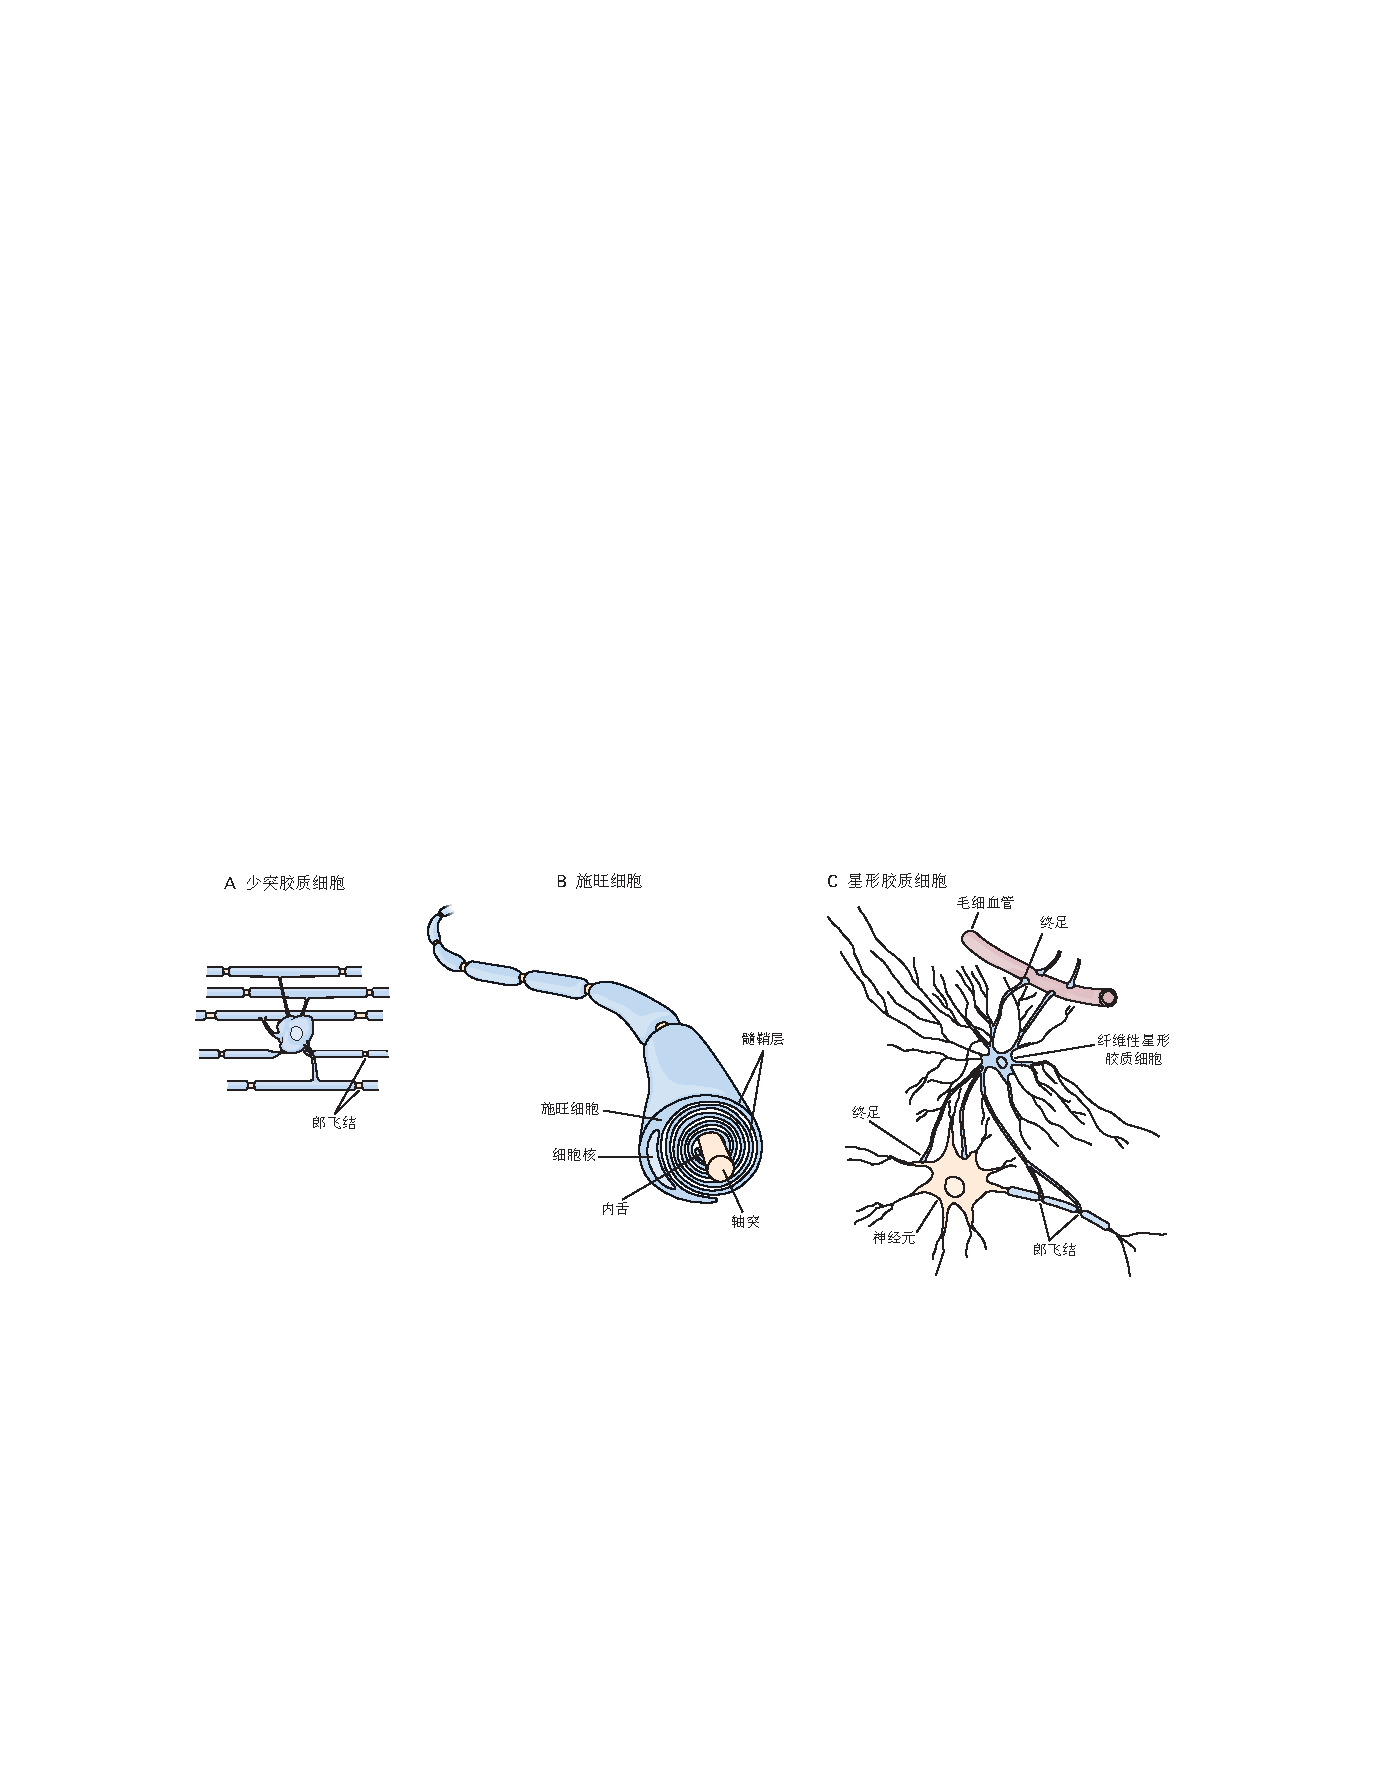
\includegraphics[width=1.0\linewidth]{chap07/fig_7_1}
	\caption{神经胶质细胞的主要类型是中枢神经系统中的少突胶质细胞和星形胶质细胞以及周围神经系统中的\textit{施旺细胞}。
		A. \textit{少突胶质细胞}是突起相对较少的小细胞。
		如图所示,在大脑的白质中,它们提供了隔离轴突的髓鞘。
		单个少突胶质细胞可以将其膜状突起包裹在许多轴突周围。
		在灰质中,神经周围少突胶质细胞包围并支持神经元的细胞体。
		B. \textit{施旺细胞}为周围神经系统中的轴突提供髓鞘。
		在发育过程中,几个\textit{施旺细胞}沿着单个轴突的长度排列。
		每个细胞在\textit{郎飞结}的 2 个节点之间形成一个大约 1 毫米长的髓鞘。
		髓鞘由\textit{施旺细胞}的内舌围绕轴突旋转数圈形成,将轴突包裹在膜层中。
		实际上,髓磷脂层比这里显示的更紧凑。
		C. \textit{星形胶质细胞}是中枢神经系统中的一类主要神经胶质细胞,其特征在于其星形形状和突起上的\textit{终足}。
		因为这些\textit{终足}使星形胶质细胞与毛细血管和神经元接触,所以星形胶质细胞被认为具有营养功能。
		星形胶质细胞在维持血脑屏障方面也起着重要作用(在本章后面描述)。}
	\label{fig:7_1}
\end{figure}


\section{神经元和胶质细胞具有许多结构和分子特征}

如图~\ref{fig:7_2}~所示,神经元和胶质细胞由胚胎神经系统的共同神经上皮祖细胞发育而来,并具有许多相同的结构特征。
这些细胞的边界由细胞膜或\textit{细胞质膜}界定。
神经细胞膜具有所有生物膜的一般不对称双层结构,是大多数水溶性物质不可渗透的疏水屏障。
细胞质有 2 个主要成分:胞质溶胶和膜状细胞器。


\begin{figure}[htbp]
	\centering
	\includegraphics[width=0.6\linewidth]{chap07/fig_7_2}
	\caption{神经元的结构。
		脊髓运动神经元的细胞体和细胞核被双层膜包围(即核膜),与内质网相连。
		构成核膜的 2 个膜层之间的空间与内质网的腔连续。
		树突从神经元的基底面出现,轴突从顶端面出现\cite{williams1989bannister}。}
	\label{fig:7_2}
\end{figure}


% Cytosol is the aqueous phase of cytoplasm
胞质溶胶是细胞质的水相。
在此阶段,实际上只有少数蛋白质游离在溶液中。
除了一些催化代谢反应的酶外,大多数蛋白质都被组织成功能复合物。
最近一个叫做蛋白质组学的分支学科已经确定这些复合物可以由许多不同的蛋白质组成,其中没有任何一种蛋白质与另一种蛋白质共价连接。
例如,\textit{N-甲基-D-天冬氨酸}型谷氨酸受体(一种介导中枢神经系统兴奋性突触传递的膜相关蛋白)的细胞质尾部锚定在由 100 多种支架蛋白组成的大型复合体中(将在后面的章节中讨论:许多参与第二信使信号转导的胞质蛋白,它们嵌入\textit{细胞质膜}正下方的细胞骨架基质中)。
核糖体是翻译\textit{信使核糖核酸}分子的细胞器,由几个蛋白质亚基组成。
蛋白酶体是一种大型多酶细胞器,可降解泛素化蛋白质(本章稍后描述的过程),它也存在于神经元和胶质细胞的胞质溶胶中。


膜细胞器是细胞质的第二个主要成分,包括线粒体和过氧化物酶体,以及一个由小管、囊泡和空泡组成复杂系统,即液泡系统。
线粒体和过氧化物酶体处理分子氧。
线粒体产生\textit{三磷酸腺苷},这是细胞能量转移或消耗的主要分子,而过氧化物酶体可防止强氧化剂过氧化氢的积累。
线粒体源自在进化早期侵入真核细胞的共生古细菌,在功能上与液泡系统不连续。
线粒体还在 \ce{Ca^2+} 稳态和脂质生物合成中发挥其他重要作用。


如图~\ref{fig:7_3}~所示,液泡器包括光滑内质网、粗面内质网、高尔基复合体、分泌小泡、核内体、溶酶体,以及连接这些不同隔室的多种运输小泡。
它们的管腔在拓扑上对应于细胞的外部;
因此,它们脂质双层的内层小叶对应于\textit{细胞质膜}的外层小叶。


\begin{figure}[htbp]
	\centering
	\includegraphics[width=1.0\linewidth]{chap07/fig_7_3}
	\caption{神经元的细胞器。
		电子显微照片显示神经元 4 个不同区域的细胞质\cite{peters1991neuropil}。
		A. 树突从锥体神经元的细胞体中出现,其中包括\textit{细胞核}上方的\textit{内质网}和\textit{高尔基复合体}附近的一部分。
		一些\textit{高尔基间隙}已进入树突,\textit{线粒体}、\textit{溶酶体}和\textit{核糖体}也已进入。
		\textit{微管}是细胞质中突出的细胞骨架丝。
		在顶部和右侧可以看到与树突接触的\textit{轴突末梢}。
		B. 参与大分子合成的脊髓运动神经元的某些成分。
		\textit{细胞核}含有大量\textit{染色质},并以含有许多核孔(箭头)的核膜为界。
		\textit{信使核糖核酸}通过这些孔离开细胞核并附着在核糖体上,核糖体在细胞质中保持游离状态或附着在内质网膜上形成\textit{粗面内质网}。
		细胞质中合成的调节蛋白通过孔进入细胞核。
		可以看到\textit{高尔基体}的几个部分,以及\textit{溶酶体}和\textit{线粒体}。
		\textit{C、D.} 背根神经节细胞(C)和运动神经元(D)的显微照片显示了细胞体中主要负责蛋白质合成和加工的细胞器。
		\textit{信使核糖核酸}通过核膜进入细胞质并被翻译成蛋白质。
		游离多核糖体(即附着在单个\textit{信使核糖核酸}上的 1 串核糖体)产生胞质蛋白和被导入\textit{线粒体}和过氧化物酶体中的蛋白。
		多核糖体附着于\textit{内质网}膜后,会形成以内质网为目的地的蛋白质。
		此处显示的运动神经元的特定区域还包括\textit{高尔基体}的膜,其中进一步处理膜和分泌蛋白。
		一些新合成的蛋白质在小泡中离开高尔基体,小泡沿着轴突向下移动到突触;
		其他膜蛋白被掺入\textit{溶酶体}和其他膜细胞器中。
		\textit{微管}和\textit{神经细丝}是细胞骨架的组成部分。}
	\label{fig:7_3}
\end{figure}


% The major subcompartments
这些区域并不连接在一起,但在功能上仍有联系,因为膜质和腔质材料通过运输囊泡从一个区域移到另一个区域。
例如,在\textit{粗面内质网}(布满核糖体的网状部分)和光滑内质网中合成的蛋白质和磷脂被运送到高尔基复合体,然后进入分泌小泡,在小泡膜与质膜融合时释放其内容物(这个过程称为\textit{胞吐})。
这种分泌途径将膜成分添加到\textit{细胞质膜},并将这些分泌囊泡的内容物释放到细胞外空间。


相反,细胞膜的成分通过内吞囊泡进入细胞(内吞作用)。
这些被纳入早期内体,分选集中在细胞外围的隔室。
内吞膜通常含有特定的蛋白质(如跨膜受体)可以通过成熟为循环核内体而直接回到\textit{细胞质膜},也可以成熟为晚期核内体,后者通过与溶酶体融合而被靶向降解(胞吐作用和胞吞作用将在本章后面详细讨论)。
平滑内质网还储存拥有调节神经元作用的\ce{Ca^2+}(参见第~\ref{chap:chap14}~章中关于~\ce{Ca^2+} 释放的讨论)。


如图~\ref{fig:7_3}~所示,粗面内质网的一个特殊部分形成了核包膜,这是一个球形扁平腔,围绕着染色体\textit{脱氧核糖核酸}及其相关蛋白(组蛋白、转录因子、聚合酶和异构酶)并界定细胞核。
因为核包膜与内质网的其他部分和液泡器的其他膜是连续的,所以推测它是作为\textit{细胞质膜}的内陷进化而来的,用于包裹真核染色体。
核膜被核孔打断,核膜的内外膜融合导致亲水通道的形成,蛋白质和\textit{核糖核酸}通过该通道在细胞质本身和核细胞质之间交换。


尽管核质和细胞质是细胞质的连续结构域,但只有分子量小于 5 千的分子才能通过扩散自由地穿过核孔。
较大的分子需要帮助。
一些蛋白质具有特殊的核定位信号,这些区域由一系列基本氨基酸(精氨酸和赖氨酸)组成,可被称为\textit{核输入受体}的可溶性蛋白质识别。
在核孔中,这种复合物被另一组称为核孔蛋白的蛋白质引导进入细胞核。


神经细胞体的细胞质延伸到树突状树中,没有功能分化。 
通常,细胞体细胞质中的所有细胞器也存在于树突中,尽管粗面内质网、高尔基复合体和溶酶体的密度随着与细胞体的距离而迅速减小。 
如图~\ref{fig:7_4}~和图~\ref{fig:7_5}~所示在树突中,光滑的内质网在称为棘的细突底部突出,这是兴奋性突触的接受部分。
树突棘中多聚核糖体的浓度介导局部蛋白质合成(见下文)。


\begin{figure}[htbp]
	\centering
	\includegraphics[width=0.87\linewidth]{chap07/fig_7_4}
	\caption{高尔基体和内质网膜从细胞体延伸到树突中。
		A. 高尔基体复合体(实线箭头)在光学显微镜下显示为数条伸入树突(空心箭头)但未伸入轴突的细丝。
		底部的箭头表示轴突小丘。
		对于这张显微照片,脑干的一个大神经元用专门针对高尔基复合体的抗体进行了免疫染色\cite{de1986heterogeneous}。
		B. 光滑的内质网(箭头)延伸到树突棘的颈部,而另一个膜室位于脊柱的起点(箭头)\cite{cooney2002endosomal}。}
	\label{fig:7_4}
\end{figure}


\begin{figure}[htbp]
	\centering
	\includegraphics[width=1.0\linewidth]{chap07/fig_7_5}
	\caption{树突棘的类型。
		海马体\textit{阿蒙角}1 区锥体细胞的成熟树突显示 3 种类型的树突棘形状。
		左图基于一系列电子显微照片\cite{harris1989dendritic,sorra1993occurrence}。
		\textit{A.} 在这个\textit{细}的树突棘中,位于突触前轴突对面的增厚的受体表面(箭头)包含突触受体。
		此处以及 B 和 C 中显示的组织来自出生后第 15 天大鼠大脑的海马体。
		B. 含有突触后密度(箭头)的\textit{粗短}棘在成熟的海马体中既小又罕见。
		它们较大的对应物(未显示)在未成熟的大脑中占主导地位。
		C. \textit{蘑菇状}树突棘的头部较大。
		此处显示的未成熟脊柱包含平滑内质网的扁平池,一些具有串珠外观(实线箭头)。
		空心箭头表示突触后密度。}
	\label{fig:7_5}
\end{figure}


与细胞体和树突的连续性相反,在轴突出现的地方,细胞体与轴突丘之间存在一个明显的功能边界。
如图~\ref{fig:7_4}~所示,构成神经元中蛋白质主要生物合成机制的细胞器(如核糖体、粗面内质网和高尔基复合体)通常不包括在轴突内,溶酶体和某些蛋白质也是如此。
然而,轴突富含光滑内质网、单个突触小泡及其前体膜。



\section{细胞骨架决定细胞形状}

细胞骨架决定细胞的形状,并且也是细胞质内细胞器分布不对称的原因。
它包括 3 种丝状结构:微管、神经丝和微丝。
这些细丝和相关蛋白约占细胞总蛋白的 1/4。


微管产生一个从神经元一端延伸到另一端的成长支架,在发育和维持细胞形状方面发挥关键作用。
单个微管可以长达 0.1 毫米。
如图~\ref{fig:7_6}A~所示,微管由原丝组成,每个原丝由多对沿微管纵向排列的 a-微管蛋白亚基和 b-微管蛋白亚基组成。
微管蛋白亚基沿原丝与相邻的亚基结合,并在相邻原丝之间横向结合。
微管具有极性,一端为正端(或生长端),一端为负端(微管可以在负端解聚)。
有趣的是,轴突和树突中的微管方向不同。
在轴突中,微管显示单一方向,正端朝向远离细胞体的方向。
在近端树突中,微管的方向可以是双向的,正端朝向或远离细胞体。


\begin{figure}[htbp]
	\centering
	\includegraphics[width=1.0\linewidth]{chap07/fig_7_6}
	\caption{纤维结构图谱。
		A. \textit{微管}是最大直径的纤维(25 纳米),是由 13 根\textit{原丝}组成的螺旋圆柱体,每根原丝的宽度为 5 纳米。
		每个原丝由一列交替的 $\alpha$-微管蛋白亚基和$\beta$-微管蛋白亚基组成;
		每个亚基的分子量约为 5 万\textit{道尔顿}。
		相邻的亚基沿纵向原丝相互结合,并在相邻原丝的亚基之间横向结合。
		微管蛋白分子是由 1 个 $\alpha$-微管蛋白亚基和 1 个 $\beta$-微管蛋白亚基组成的异二聚体。
		1. 微管视图。
		箭头指示右手螺旋的方向。
		2. 微管的侧视图显示交替的$\alpha$亚基和$\beta$亚基。
		B. \textit{神经丝}由相互缠绕的纤维构成,以产生厚度增加的线圈。
		最薄的单元是形成卷曲螺旋异二聚体的单体。
		这些二聚体形成成为原丝的四聚体复合物。
		2 个原纤维变成一个原纤维,3 个原纤维螺旋扭曲形成直径 10 纳米的神经丝\cite{bershadsky2012cytoskeleton}。
		C. \textit{微丝}是直径最小的纤维(约 7 纳米),由排列成螺旋状的两股聚合\textit{球状肌动蛋白}单体组成。
		在哺乳动物中至少发现了6 种不同(但密切相关)的肌动蛋白;
		每个变体都由一个单独的基因编码。
		微丝是极性结构,因为球状单体是不对称的。}
	\label{fig:7_6}
\end{figure}


微管通过在其正端添加\textit{三磷酸鸟苷}结合的微管蛋白二聚体来生长。
聚合后不久,\textit{三磷酸鸟苷}被水解为\textit{二磷酸鸟苷}。
当微管停止生长时,其正端被\textit{二磷酸鸟苷}结合的微管蛋白单体所覆盖。
\textit{二磷酸鸟苷}结合的微管蛋白对聚合物的低亲和力会导致灾难性的解聚,除非微管通过与其他蛋白的相互作用而稳定下来。


事实上,虽然微管在分裂细胞中经历聚合和解聚的快速循环,这种现象被称为动态不稳定,但在成熟的树突和轴突中,它们要稳定得多。
这种稳定性是由\textit{微管相关蛋白}实现的,它促进了微管蛋白聚合物的定向聚合和组装。
轴突中的\textit{微管相关蛋白}不同于树突中的\textit{微管相关蛋白}。
例如,\textit{微管相关蛋白}2 存在于树突中,但不存在于轴突中,轴突中存在 tau 蛋白(见文本框~\ref{box:7_1})和\textit{微管相关蛋白}1b。
此外,微管稳定性也受到许多不同类型的可逆微管蛋白翻译后修饰的严格调节,例如乙酰化、去酪氨酸化和聚谷氨酰化。
在阿尔茨海默病和其他一些退行性疾病中,tau 蛋白被修饰并异常聚合,形成一种称为神经原纤维缠结的特征性损伤(文本框~\ref{box:7_1})。


\begin{proposition}[神经解剖学导航术语] \label{box:7_1}
	
	\quad \quad 蛋白质的异常积累是许多神经系统疾病的标志。
	
	\quad \quad Tau蛋白是一种微管结合蛋白,通常存在于神经细胞中。
	在阿尔茨海默病中,在光学显微镜下,神经元、神经胶质细胞以及细胞外空间中都可以看到tau的异常聚集。
	如图~\ref{fig:7_7}A~和第~\ref{chap:chap64}~章所示,排列在细长聚合物中的高度磷酸化的tau分子相互缠绕,形成成对的螺旋丝。
	如图~\ref{fig:7_7}A~所示,被称为神经原纤维缠结的聚合物束聚集在神经元细胞体、树突和轴突中。
	
	\quad \quad 在正常神经元中,tau要么与微管结合,要么在胞质溶胶中游离。
	在缠结中,它不与微管结合,但高度不溶。
	缠结的形成至少部分是因为tau没有被蛋白经酶解作用而降解。
	堆积物干扰微管蛋白的聚合,从而干扰轴突运输。
	因此,神经元的形状没有得到维持。
	
	\quad \quad 在\textit{进行性核上性麻痹}(一种运动障碍)患者和\textit{额颞痴呆}(一组影响额叶和颞叶的神经退行性疾病)患者的神经元中也发现了Tau积聚(第~\ref{chap:chap63}~章)。
	\textit{额颞痴呆}的家族形式是由tau基因突变引起的。
	在\textit{进行性核上性麻痹}、皮层-基底神经节变性和\textit{额颞痴呆}的星形胶质细胞和少突胶质细胞中也发现异常聚集体。
	
	\quad \quad 如图~\ref{fig:7_7}B和第~\ref{chap:chap64}~章所示,$\beta$淀粉样蛋白肽也在阿尔茨海默病的细胞外空间积聚。
	它是一种更大的整体膜蛋白淀粉样蛋白前体蛋白的小蛋白水解产物,通常由与细胞内膜相关的几种蛋白水解酶处理。
	产生$\beta$-淀粉样蛋白的蛋白水解途径需要$\beta$-分泌酶。
	
	\quad \quad 由于未知的原因,在阿尔茨海默病中,异常量的淀粉样蛋白前体由$\beta$-分泌酶处理。
	一些早发性家族性阿尔茨海默病患者的淀粉样蛋白前体基因或编码膜蛋白早老素1和2的基因发生突变,这些基因与分泌酶活性密切相关。
	
	\quad \quad 如图~\ref{fig:7_7}C和第~\ref{chap:chap63}~章所示,在帕金森病中,$\alpha$-突触核蛋白的异常聚集体在神经元的细胞体中积累。
	与tau一样,a-突触核蛋白是细胞的一种正常可溶性成分。
	但在帕金森病中,它变得不溶,形成称为路易体的球形内含物。
	
	\quad \quad 这些异常内含物也含有泛素。
	由于泛素是蛋白质蛋白酶体降解所必需的,它的存在表明受影响的神经元试图靶向$\alpha$-突触核蛋白或其他分子成分进行蛋白水解。
	显然,降解不会发生,可能是因为蛋白质的错误折叠或异常聚集,或者是因为细胞中错误的蛋白水解处理。
	
	\quad \quad 这些异常的蛋白质积累会影响神经元和神经胶质细胞的生理机能吗?
	一方面,积累可以响应蛋白质的翻译后处理的改变而形成,并用于分离异常蛋白质,从而允许正常的细胞活动。
	另一方面,这些积累可能会破坏细胞活动,如膜运输、轴突和树突运输,以及特定类别神经元之间突触连接的维持。
	此外,除了聚集之外,改变的蛋白质本身可能具有有害影响。
	对于$\beta$-淀粉样蛋白,有证据表明该肽本身具有毒性。
	
\end{proposition}


\begin{figure}[htbp]
	\centering
	\includegraphics[width=0.8\linewidth]{chap07/fig_7_7}
	\caption{阿尔茨海默病和帕金森病神经元内蛋白质的异常聚集。
	A. 左图:阿尔茨海默病的细胞内神经原纤维缠结,此处用暗银染色。
	右图:缠结的电子显微照片显示,异常细丝成束,充满树突。
	细丝由改变的tau蛋白组成。
	B. 在阿尔茨海默病中,\textit{淀粉状蛋白斑}由聚合的$\beta$-淀粉样肽的细胞外沉积形成。
	此处显示的斑块有一个致密的淀粉样蛋白核心,以及周围的沉积物晕。
	斑块中的一些神经元过程表现出缠结病理。
	C. 帕金森病患者黑质中的路易体含有由$\alpha$-突触核蛋白和其他蛋白质组成的异常细丝。}
	\label{fig:7_7}
\end{figure}


微管蛋白由多基因家族编码。
至少有 6 个基因编码 $\alpha$ 亚基和 $\beta$ 亚基。
由于不同基因的表达或转录后修饰,大脑中存在 20 多种微管蛋白亚型。


如图~\ref{fig:7_6}B~所示,直径为 10 纳米的神经丝是细胞骨架的骨骼。
神经丝与其他细胞类型的中间丝有关,包括上皮细胞(头发和指甲)的细胞角蛋白、星形胶质细胞中的神经胶质原纤维酸性蛋白和肌肉中的结蛋白。
与微管不同,神经丝是稳定的并且几乎完全聚合在细胞中。


如图~\ref{fig:7_6}C~所示,微丝的直径为 3 纳米至 7 纳米,是构成细胞骨架的 3 种主要纤维类型中最细的。
与肌肉的细丝一样,微丝由两股聚合的球状肌动蛋白单体组成,每条单体都带有\textit{三磷酸腺苷}或\textit{二磷酸腺苷},缠绕成双链螺旋。
肌动蛋白是所有细胞的主要成分,可能是自然界中最丰富的动物蛋白。
有几种密切相关的分子形式:骨骼肌的 $\alpha$ 肌动蛋白和至少 2 种其他分子形式($\beta$ 和$\gamma$)。
每个都由不同的基因编码。
高等脊椎动物的神经肌动蛋白是 $\beta$ 和$\gamma$种类的混合物,它与肌肉肌动蛋白的区别在于几个氨基酸残基。 
大多数肌动蛋白分子是高度保守的,不仅在一个物种的不同细胞类型中,而且在人类和原生动物等远亲生物中也是如此。


% Unlike microtubules and neurofilaments
与微管和神经丝不同,肌动蛋白丝很短。
它们集中在细胞外围的皮层细胞质中,就在\textit{细胞质膜}下面,在那里它们与许多肌动蛋白结合蛋白(例如,\textit{血影蛋白-胞影蛋白}、\textit{锚定蛋白}、\textit{踝蛋白}和\textit{辅肌动蛋白})形成致密网络。
该基质在细胞外围的动态功能中起着关键作用,例如发育过程中生长锥(轴突的生长尖端)的运动、细胞表面特化微域的产生以及突触前后神经形态的特化。


% Like microtubules, microfilaments undergo
与微管一样,微丝经历聚合和解聚循环。
在任何时候,细胞中大约一半总肌动蛋白可以作为未聚合的单体存在。
肌动蛋白的状态由结合蛋白控制,结合蛋白通过覆盖快速生长的细丝末端或切断它来促进组装并限制聚合物长度。 
其他结合蛋白交联或束缚肌动蛋白丝。
微管和微丝的动态状态允许成熟的神经元收缩旧的轴突和树突,并延伸新的轴突和树突。
这种结构可塑性被认为是突触连接和功效变化的主要因素,因此也是长期记忆和学习的细胞机制。


% In addition to serving as the cytoskeleton
除了充当细胞骨架外,微管和肌动蛋白丝还充当轨道,分子马达沿着轨道快速驱动细胞器和蛋白质。
肌动蛋白丝使用的马达(肌球蛋白)还介导其他类型的细胞运动,包括细胞突起的延伸和膜状细胞器从大部分细胞质转移到质膜附近的区域(肌动球蛋白负责肌肉收缩)。
由于微管和肌动蛋白丝是极性的,每个马达只能向一个方向驱动其细胞器货物。


如前所述,微管在轴突中平行排列,正端指向远离细胞体的方向,负端朝向细胞体。
如图~\ref{fig:7_8}~所示,这种规则的方向允许一些细胞器向神经末梢移动,而另一些细胞器则远离神经末梢,方向由特定类型的分子马达决定,从而保持了轴突细胞器的独特分布。
然而,在树突中,极性相反的微管混合在一起,这解释了为什么细胞体和树突的细胞器相似。




\section{蛋白质颗粒和细胞器沿轴突和树突主动运输}

在神经元中,大多数蛋白质在细胞体中由\textit{信使核糖核酸}制成,比如神经递质的生物合成酶、突触小泡膜的一些组成部分和神经内分泌多肽。
由于轴突和末端通常距离细胞体很远,因此维持这些偏远区域的功能是一项挑战。
被动扩散的速度太慢,无法将囊泡、颗粒甚至单个大分子输送到如此远的距离。


轴突末端是分泌神经递质的部位,离细胞体特别远。
在支配人类腿部肌肉的运动神经元中,神经末梢与细胞体的距离可以超过细胞体直径的 1 万倍。
因此,如图~\ref{fig:7_9}~所示,在细胞体内形成的膜和分泌物必须通过主动运输到达轴突末端。


\begin{figure}[htbp]
	\centering
	\includegraphics[width=0.65\linewidth]{chap07/fig_7_9}
	\caption{神经元中的膜运输。
		1. 分泌细胞器的蛋白质和脂质在内质网中合成并转运到高尔基复合体,在那里组装大的致密核心囊泡(含肽分泌颗粒)和突触囊泡前体。
		2. 大的致密核心囊泡和运输囊泡通过轴突运输将突触囊泡蛋白沿轴突向下传送。
		3. 在神经末梢,突触小泡组装并装载非肽类神经递质。
		突触小泡和大的致密核小泡通过胞吐作用释放其内容物。
		4. 胞吐作用后,大的致密核囊泡膜返回细胞体以供再利用或降解。
		突触小泡膜在突触前末梢经历多次局部胞吐和胞吞循环。}
	\label{fig:7_9}
\end{figure}


1948 年,\textit{保罗$\cdot$韦斯}第一次证明了轴突运输,当时他绑住了一根坐骨神经,并观察到神经中的轴浆随着时间的推移在结扎线的近端聚集。
他的结论是:轴浆以一个缓慢而恒定的速度从细胞体向细胞末端移动,他将这一过程称为\textit{轴浆流}。
如今我们知道,\textit{韦斯}观察到的轴浆流动由 2 种不同的机制组成,一种是快速机制,另一种是慢速机制。


膜状细胞器通过快速轴突运输向轴突末端(顺行方向)移动并返回细胞体(逆行方向),这种运输形式在恒温动物体内每天可达 400 毫米。
相比之下,细胞溶质和细胞骨架蛋白只能通过更慢的运输形式(轴突运输)沿顺行方向移动。
神经元中的这些运输机制是对所有分泌细胞中一种促进细胞器胞内运动过程的适应。
由于所有这些运输机制都是沿着轴突进行的,因此神经解剖学家已经利用这些机制来追踪单个轴突的运动轨迹以及神经元之间的相互联系(文本框~\ref{box:7_2})。

\begin{proposition}[利用轴突运输进行神经解剖学追踪] \label{box:7_2}
	
	\quad \quad 神经解剖学家通常通过以下方法来定位特定神经细胞体的轴突和末梢:
	显微注射染料;
	表达荧光蛋白;
	或在给予放射性标记的氨基酸、某些标记的糖(\textit{岩藻糖}或氨基糖,糖蛋白的前体)或特异性递质物质后不久用放射自显影法追踪特定蛋白质。
	
	\quad \quad 同样,通过内吞作用在神经末梢吸收并运回细胞体的微粒、蛋白质或染料也可用于识别细胞体。
	\textit{辣根过氧化物酶}在这类研究中应用最为广泛,因为它很容易进行逆行运输,并且它的反应产物也可以很容易地通过组织化学方法被观察到。
	
	\quad \quad 如图~\ref{fig:7_10}~所示,神经解剖学家还利用轴突运输来标记神经元之间交换的物质,从而识别神经元网络。
	
\end{proposition}


\begin{figure}[htbp]
	\centering
	\includegraphics[width=1.0\linewidth]{chap07/fig_7_10}
	\caption{\textit{单纯疱疹病毒}的轴索转运被用来追踪猴子的皮层通路。
		根据毒株的不同,病毒通过轴突运输沿顺行方向或逆行方向移动。
		在任何一个方向上,它都会进入一个神经元,受感染的细胞与该神经元进行突触接触。
		在这里,使用顺行移动菌株(\textit{单纯疱疹病毒}-1型H129株)追踪猴子\textit{初级运动皮层}中的细胞向\textit{小脑}的投射。
		注射到猴子控制手臂的\textit{初级运动皮层}区域。
		4天后,对大脑进行切片并对病毒抗原进行免疫染色。
		显微照片显示,病毒从初级运动皮层转移到\textit{脑桥核}的二阶神经元(A),然后转移到\textit{小脑皮层}的三阶神经元(B)。}
	\label{fig:7_10}
\end{figure}



\subsection{\textit{快速轴突运输}携带膜细胞器}

如图~\ref{fig:7_11}~所示,大型膜状细胞器通过快速运输进出轴突末端。
这些细胞器包括突触小泡前体、大的致密核心小泡、线粒体、光滑内质网的元素和携带\textit{核糖核酸}的蛋白质颗粒。
直接显微分析表明,快速运输是以停止和开始(跳跃式)的方式,沿着与轴突主轴对齐的微管线性轨道进行的。
快速运输的跳跃性质是由于细胞器会周期性地从轨道上分离,或会与其他微粒碰撞所致。


\begin{figure}[htbp]
	\centering
	\includegraphics[width=1.0\linewidth]{chap07/fig_7_11}
	\caption{早期关于顺行轴突运输的实验使用了蛋白质的放射性标记。
		在这里说明的实验中,在将 [$^3$H]-亮氨酸注射到脊髓腰部背根神经节后,在不同时间测量了放射性蛋白沿猫坐骨神经的分布。
		为了在一张图中显示不同时间(注射后 2、4、6、8 和 10 小时)的传输曲线,使用了多个纵坐标标度(以对数单位表示)。
		大量标记蛋白留在神经节细胞体中,但随着时间的推移,沿着坐骨神经中的轴突移出,因此标记蛋白的前进前沿逐渐远离细胞体(箭头)。
		运输速度可以根据不同时间前沿的距离来计算。
		通过此类实验,\textit{西德尼$\cdot$奥克斯}发现,在人体正常体温下,\textit{快速轴突运输}的速度恒定为每天 410 毫米\cite{ochs1972fast}。}
	\label{fig:7_11}
\end{figure}


早期的背根神经节细胞实验表明,顺行快速运输严重依赖于\textit{三磷酸腺苷},不受蛋白质合成抑制剂的影响(一旦注射的标记氨基酸被结合),并且不依赖于细胞体,因为它发生在与细胞体切断的轴突中。
事实上,主动运输可以发生在重组的无细胞轴突中。


微管提供了一个基本固定的轨道,特定的细胞器可以在这个轨道上通过分子马达进行移动。
某些生物碱会破坏微管并阻断依赖于微管的有丝分裂,它们也会干扰快速运输,由此便产生了微管参与快速轴突运输的想法。


如图~\ref{fig:7_8}~所示,分子马达最早在电子显微镜下作为微管和运动粒子之间的\textit{交叉桥}被观察到。
更先进的荧光延时显微镜技术能够观察特定载体(如线粒体和突触小泡)的轴突运输动态。
用于顺行运输的分子马达是由驱动蛋白和多种驱动蛋白的相关蛋白提供的。
驱动蛋白代表一大类\textit{三磷酸腺苷酶},每一种都运输不同的货物。
驱动蛋白是一种由两条重链和两条轻链组成的异四聚体。
每条重链具有 3 个结构域:
(1)一个球状头部(\textit{三磷酸腺苷酶}结构域),当连接到微管时充当马达,
(2)一个卷曲螺旋茎,负责与另一条重链二聚化,以及
(3)与轻链相互作用的扇形羧基末端。
复合物的这一端间接附着到细胞器,细胞器通过称为货物适配器的特定蛋白质家族移动。


\begin{figure}[htbp]
	\centering
	\includegraphics[width=1.0\linewidth]{chap07/fig_7_8}
	\caption{轴突的细胞骨架结构。
		显微照片显示了由\textit{交叉桥}(箭头)连接的微管和神经丝的密集堆积。
		细胞器在富含微管的区域中沿顺行方向运输和逆行方向运输。
		显微照片中的可视化是通过快速冷冻和深度蚀刻实现的\cite{schnapp1982cytoplasmic}。}
	\label{fig:7_8}
\end{figure}


% Fast retrograde transport primarily
快速逆行运输主要运输由神经末梢、线粒体和内质网元件的胞吞作用产生的核内体。
这些成分中的许多会通过与溶酶体融合而被分解。
快速逆行运输还传递调节神经元细胞核中基因表达的信号。
例如,神经末梢处激活的生长因子受体被吸收到囊泡中,并沿着轴突运回细胞核。
转录因子的转运通知细胞核中的基因转录装置周围的条件。
这些分子的逆行运输在神经再生和轴突再生过程中尤为重要(第~\ref{chap:chap47}~章)。 
某些毒素(破伤风毒素)以及病原体(\textit{单纯疱疹病毒}、狂犬病病毒和脊髓灰质炎病毒)也沿着轴突向细胞体输送。


% The rate of retrograde fast transport
逆行快速运输的速度大约是顺行快速运输的 1/2 到 2/3。
与顺行运输一样,分子微粒在逆行运输时也会沿着微管移动。
逆行轴突运输的\textit{马达分子}是负端定向的马达,称为\textit{动力蛋白},类似于在非神经元细胞的纤毛和鞭毛中发现的马达。
它们由一个多聚体\textit{三磷酸腺苷酶}蛋白复合物组成,2 个球状头部位于 2 个与基底结构相连的柄上。
球妆头部附着在微管上并充当马达,向聚合物的负端移动。
与驱动蛋白一样,复合体的另一端通过专门的货物适配器连接到运输的细胞器上。


% Microtubules also mediate anterograde
微管还能介导\textit{信使核糖核酸}和核糖体\textit{核糖核酸}的顺向和逆向运输,这些\textit{核糖核酸}和核糖体\textit{核糖核酸}由\textit{核糖核酸}结合蛋白形成的颗粒携带。
这些蛋白质在脊椎动物和无脊椎动物的神经系统中都有表征,包括\textit{胞质聚腺苷酸化元件结合蛋白}、脆性 X 蛋白、Hu 蛋白、NOVA 和\textit{双链核糖核酸结合蛋白}。
这些蛋白质的活性至关重要。
例如,\textit{胞质聚腺苷酸化元件结合蛋白}在从细胞体到神经末梢的运输过程中使选定的\textit{信使核糖核酸}保持休眠状态;
一旦到达那里(受到刺激),结合蛋白可以通过介导聚腺苷酸化和信使激活来促进\textit{核糖核酸}的局部翻译。
\textit{胞质聚腺苷酸化元件结合蛋白}和\textit{双链核糖核酸结合蛋白}都是在果蝇中发现的,它们在未受精的卵中保持母体\textit{信使核糖核酸}休眠,并在受精后将\textit{信使核糖核酸}分布和定位到分裂胚胎的各个区域。
脆性 X 基因的功能缺失突变会导致严重的精神发育迟滞。


如图~\ref{fig:7_12}~所示,蛋白质、核糖体和\textit{信使核糖核酸}集中在一些树突棘的底部。
只有一组选定的\textit{信使核糖核酸}从胞体转运到树突中。
这些\textit{信使核糖核酸}包括编码肌动蛋白和细胞骨架相关蛋白、\textit{微管相关蛋白}2 和\ce{Ca^2+}/钙调蛋白依赖性蛋白激酶的$\alpha$ 亚基的\textit{信使核糖核酸}。
它们在树突中翻译以响应突触前神经元中的活动。
这种局部蛋白质的合成被认为是维持突触处分子变化的重要因素,而突触处的分子变化正是长期记忆和学习的基础。
同样,髓鞘碱性蛋白的\textit{信使核糖核酸}被运送到少突胶质细胞的远端,在那里它随着髓鞘的生长而被翻译,这将在本章后面讨论。


\begin{figure}[htbp]
	\centering
	\includegraphics[width=1.0\linewidth]{chap07/fig_7_12}
	\caption{树突状分枝中的核糖体。
		A. 一些核糖体从细胞体分派到树突,在那里它们用于局部蛋白质合成。
		这张放射自显影图显示了\textit{核糖体核糖核酸}在使用原位杂交的低密度培养物中海马神经元中的分布。
		该图像是用暗场照明制作的,其中银颗粒反射光线,因此看起来像亮点。
		表示\textit{核糖体核糖核酸}的银粒高度集中在细胞体和树突上,但在树突之间纵横交错的轴突上检测不到。
		B. 树突中的核糖体选择性地集中在脊柱和主树突轴(箭头)的交界处,在这里脊柱接触突触前神经元的轴突末端。
		这张电子显微照片显示了海马齿状回中一个神经元的蘑菇状脊柱。
		注意树突轴中没有核糖体。
		图中\textit{树突}为含有长线粒体的树突主轴放大 60,000 倍。}
	\label{fig:7_12}
\end{figure}


\subsection{\textit{慢速轴突运输}携带细胞溶质蛋白和细胞骨架的元素}

细胞溶质蛋白和细胞骨架蛋白通过\textit{慢速轴突运输}从细胞体中运出。
慢速运输只发生在顺行方向,由至少 2 个以不同速率携带不同蛋白质的动力学成分组成。


较慢的成分每天移动 0.2 毫米至 2.5 毫米,并携带构成细胞骨架纤维状元素的蛋白质:
神经丝的亚基和微管的 $\alpha$-微管蛋白亚基和 $\beta$-微管蛋白亚基。
这些纤维蛋白约占较慢成分中移动的总蛋白的 75\%。 
微管通过涉及微管滑动的机制以聚合形式运输,在这种机制中,相对较短的预组装微管沿着现有微管移动。
神经丝单体或短聚合物会被动地与微管一起移动,因为它们通过蛋白质桥交联在一起。


\textit{慢速轴突运输}的另一个组成部分的速度大约是较慢部分的两倍。
它携带凝乳蛋白、肌动蛋白和肌动蛋白结合蛋白以及多种酶和其他蛋白质。



\section{与其他分泌细胞一样,蛋白质也是在神经元中制造的}

\subsection{分泌蛋白和膜蛋白在内质网中合成和修饰}

分泌蛋白和膜蛋白的\textit{信使核糖核酸}通过粗面内质网的膜进行翻译,其多肽产物在内质网腔内广泛加工。
大多数要成为蛋白质的多肽在合成过程中都会跨过粗面内质网的膜进行转运,这一过程称为\textit{翻译转运同步机制}。


如图~\ref{fig:7_13}~所示,多肽之所以能够进行转运,是因为合成蛋白质的核糖体附着在网状细胞的膜表面。
多肽链完全转移到网状细胞腔中时,会产生一种分泌蛋白(网状细胞的内部与细胞的外部有关)。
神经活性肽就是一个重要的例子。
如果转移不完全,则会产生完整的膜蛋白。
由于多肽链在合成过程中可以多次穿过膜,因此根据蛋白质的一级氨基酸序列,多肽链可能有几种不同的跨膜结构。
神经递质受体和离子通道就是重要的例子(第~\ref{chap:chap8}~章)。


\begin{figure}[htbp]
	\centering
	\includegraphics[width=1.0\linewidth]{chap07/fig_7_13}
	\caption{\textit{内质网}中的蛋白质合成。
		游离和膜结合的\textit{多核糖体}翻译\textit{信使核糖核酸},该信使核糖核酸编码具有多种目的地的蛋白质。
		信使核糖核酸从神经元细胞核中的基因组\textit{脱氧核糖核酸}转录而来,通过细胞\textit{核孔}进入细胞质,形成多核糖体(见放大图)。
		变成分泌蛋白和膜蛋白的多肽在\textit{粗糙内质网}的膜上转运。}
	\label{fig:7_13}
\end{figure}


一些被运输到内质网中的蛋白质会留在那里。
其他蛋白质则会移动到液泡器的其他隔室或\textit{细胞质膜},或被分泌到细胞外。
在内质网中加工的蛋白质会被广泛修饰。
其中一个重要的修饰是由成对的游离巯基侧链氧化,而引起的分子内\textit{二硫键}的形成,这一过程不能发生在胞质溶胶的还原环境中。
\textit{二硫键}对于这些蛋白质的三级结构至关重要。


蛋白质可以在合成过程中(共翻译修饰)或之后(翻译后修饰)被胞质酶修饰。
其中一个例子是 N-酰化,即将酰基转移到生长中的多肽链的 N-末端。
14-碳脂肪酸肉豆蔻酰基的酰化作用可以让蛋白质通过脂质链锚定在膜上。


其他脂肪酸可以与半胱氨酸的巯基结合,产生\textit{硫代酰化}:

异戊二烯化是另一种翻译后修饰,对于将蛋白质锚定到细胞膜的胞质侧很重要。
它发生在蛋白质合成完成后不久,涉及一系列酶促步骤,通过 2 个长链疏水性多异戊烯基(具有 15 个碳原子的\textit{法尼基}或具有 20 个碳原子的\textit{香叶基}-\textit{香叶基})中的一个,对蛋白质 C 端半胱氨酸的巯基进行硫代酰化。


一些翻译后修饰很容易被逆转,因此被用来短暂地调节蛋白质的功能。
这些修饰中最常见的是蛋白激酶对丝氨酸、苏氨酸或酪氨酸残基中羟基的磷酸化。
去磷酸化由蛋白磷酸酶催化(这些反应在第~\ref{chap:chap14}~章中讨论)。
与所有翻译后修饰一样,要磷酸化的位点由要修饰的残基周围的特定氨基酸序列决定。
磷酸化能够以可逆的方式改变生理过程。
例如,蛋白质磷酸化-去磷酸化反应可以调节离子通道的动力学、转录因子的活性和细胞骨架的组装。


另一个重要的翻译后修饰是将泛素(一种具有 76 个氨基酸的高度保守的蛋白质)添加到蛋白质分子中特定赖氨酸残基的$\epsilon$-氨基上。
泛素化能调节蛋白质降解,由 3 种酶介导。
E1是一种利用\textit{三磷酸腺苷}能量的活化酶。
激活的泛素接下来被转移到结合酶 E2,然后将激活的部分转移到连接酶 E3。
E3 可以单独或与 E2 一起将泛素基转移到蛋白质的赖氨酸残基上。
特异性的产生是因为给定的蛋白质分子只能被特定的 E3,或 E3 和 E2 的组合泛素化。
一些 E3 还需要特殊的辅助因子,泛素化仅在 E3 和辅助因子蛋白存在的情况下发生。


单泛素化可以标记蛋白质,以便其在内质体-溶酶体系统中降解。
这在表面受体的内吞作用和再循环中尤为重要。
泛素基单体依次与先前添加的泛素分子中赖氨酸残基的$\epsilon$-氨基相连。
在多泛素链上添加 5 个以上的泛素后,标记蛋白质就会被蛋白酶体降解,蛋白酶体是一种大型复合物,它含有多功能蛋白酶亚基,能够将蛋白质降解成短肽。


\textit{三磷酸腺苷}-泛素-蛋白酶通路是一种对蛋白质的水解进行选择和调节的机制,它在神经元所有区域(树突、细胞体、轴突和末端)的胞质溶胶中起作用。
直到最近,人们还认为这一过程主要针对折叠不良、变性或老化受损的蛋白质发挥作用。
我们现在知道由泛素介导的蛋白水解可以受神经元活动的调节,并在突触发生和长期记忆存储等许多神经元过程中发挥特定作用。


另一个重要的蛋白质修饰是糖基化,它发生在天冬酰胺残基的氨基上(N-连接糖基化)并能够使复杂多糖链整块加入。
然后,通过由伴侣蛋白控制的一系列反应,这些多糖链会在内质网中被修剪。
其中伴侣蛋白包括热休克蛋白、钙联接蛋白和钙网蛋白。
由于寡糖分子具有很大的化学特异性,所以这些修饰对细胞功能具有重要意义。
例如,发育过程中发生的细胞间相互作用依赖于 2 个相互作用的细胞表面糖蛋白之间的分子识别。
此外,由于特定的蛋白质可能具有不同的寡糖链,故糖基化可以使蛋白质的功能多样化。
糖基化可以增加蛋白质的亲水性(对分泌蛋白有用),调节蛋白质与大分子结合的能力,并延缓蛋白质的降解。


一种有趣的\textit{信使核糖核酸}翻译后修饰是\textit{核糖核酸干扰},即双链\textit{核糖核酸}的靶向破坏。
这种机制被认为是为了保护细胞免受病毒和其他流氓核酸片段的侵害而产生的,它能够组成任何目标蛋白质的合成。 
双链\textit{核糖核酸}会被一种酶复合物吸收,这种酶复合物会将分子切割成低聚物。
\textit{核糖核酸}序列被复合物保留。
最终,任何同源杂交\textit{核糖核酸}链(无论是双链还是单链)都将被破坏。
这个过程具有再生性:复合物保留一个杂交片段,然后继续破坏另一个\textit{核糖核酸}分子,直到细胞中没有\textit{核糖核酸}分子为止。
尽管\textit{核糖核酸干扰}在正常细胞中的生理作用尚不清楚,但将\textit{核糖核酸干扰}转染或注射到细胞中具有重要的研究和临床意义(第~\ref{chap:chap2}~章)。



\subsection{分泌蛋白在高尔基复合体中被修饰}

内质网中的蛋白质通过运输囊泡被运输到高尔基复合体中,它们在高尔基复合体中被修饰,然后被转移到\textit{突触末稍}和\textit{细胞质膜}的其他部分。
高尔基复合体表现为一组膜状囊,彼此排列成长条状。


从简单的单细胞原核生物(酵母)到多细胞生物体的神经元和胶质细胞,囊泡在分泌通路和内吞通路的各个区域之间的运输机制大致相似。
运输囊泡从膜发展而来,首先是在膜的胞质表面的特定区域中组装形成衣被或衣被蛋白质。
衣被有 2 个功能:
它能够形成刚性笼状结构,使膜外翻成芽状,还能选择蛋白质并将它纳入囊泡中。


细胞有多种类型的衣被。
在内吞过程中,凝集素衣被能够协助外翻高尔基复合体膜和\textit{细胞质膜}。
另外 2 种衣被,\textit{衣被蛋白} I 和 \textit{衣被蛋白} II,会覆盖在穿梭于内质网和高尔基复合体之间的运输囊泡上。
一旦游离囊泡形成,衣被通常会迅速溶解。
囊泡与靶膜的融合由一系列分子相互作用介导,其中最重要的是 2 个相互作用膜的胞质表面上小蛋白的相互识别:
\textit{囊泡可溶性N-乙基马来酰亚胺敏感因子附着受体}和\textit{靶膜靶膜可溶性N-乙基马来酰亚胺敏感因子附着受体}。
第~\ref{chap:chap15}~章讨论了\textit{可溶性N-乙基马来酰亚胺敏感因子附着受体}蛋白通过突触小泡与\textit{细胞质膜}融合释放神经递质的作用。


来自内质网的囊泡到达高尔基复合体的顺侧(面向细胞核的一侧),并与高尔基复合体的膜融合,以将其内容物输送到高尔基复合体中。
这些蛋白质从一个高尔基体隔室(潴泡)移动到下一个隔室,从顺侧到逆侧,这之间经历了一系列的酶促反应。
每个高尔基小室或一组小室都专门用于某种特定类型的反应。
有几种类型的蛋白质修饰(其中一些始于内质网)发生在高尔基复合体内部或与其逆侧相邻的运输站内,即逆高尔基网络(高尔基复合体的逆侧通常朝向远离细胞核的轴突丘的一面)。
这些修饰包括添加 N-连接寡糖、O-连接(在丝氨酸和苏氨酸的羟基上)糖基化、磷酸化和硫酸化。


通过高尔基复合体的可溶性和膜结合蛋白都以各种囊泡的形式出现在逆高尔基网络中,这些囊泡的分子组成和目的地各不相同。
如图~\ref{fig:7_2}~所示,从逆高尔基体网络转运的蛋白质包括分泌产物以及\textit{细胞质膜}、核内体和其他膜细胞器的新合成成分。
一类囊泡携带新合成的质膜蛋白和持续分泌的蛋白质(组成型分泌)。
这些囊泡以不受控制的方式与质膜融合。
这些囊泡的一种重要类型是将溶酶体酶输送至次级内体中。


还有其他类型的囊泡携带由细胞外刺激(调节分泌)释放的分泌蛋白。
其中一种囊泡储存高浓度的分泌产物,主要是神经活性肽。
由于它们在电子显微镜下呈现出高电子密度(渗透压亲和)的特性,故被称为大密核囊泡,这些囊泡在功能和生物生成上与内分泌细胞的含肽颗粒相似。
大密核囊泡的主要目的地是轴突,但在神经元的所有区域都可以看到。
它们积聚在\textit{细胞质膜}正下方的细胞质中,并高度集中在轴突末端,在那里它们的内容物通过\ce{Ca^2+}调节的胞吐作用释放。


最近的研究表明,小突触囊泡(负责在轴突末端快速释放神经递质的电子透明小泡)作为单独的货物被主动运输到\textit{突触末稍}。
一般认为,小突触囊泡的蛋白质成分源自逆高尔基体网络的大前体小泡。
这些突触小泡已经包含了使其能够在突触前活动区融合的大部分蛋白质。
储存在这些突触小泡中的神经递质分子在\ce{Ca^2+}通过靠近释放点的通道流入的调节下,通过外泌作用释放出来。
然后,囊泡会经历第~\ref{chap:chap15}~章所述的循环/胞吐作用。
重要的是,这些囊泡会被称为囊泡转运蛋白的专门转运蛋白重新填充,这些转运蛋白对每种不同的神经递质(例如,谷氨酸、\textit{$\gamma$-氨基丁酸}、乙酰胆碱)都具有特异性。



\section{表面膜和细胞外物质在细胞内循环}

从\textit{细胞质膜}到内部细胞器的胞吞运输不断平衡着流向细胞表面的囊泡运输。
这种运输对于维持\textit{细胞质膜}表面的稳定状态至关重要。
它可以改变细胞表面许多重要调节分子的活性(例如,通过去除受体和粘附分子)。
它还将营养物质和分子(例如可消耗的受体配体和受损的膜蛋白)清除到细胞的降解区。
最后,它还能回收神经末梢的突触小泡(第~\ref{chap:chap15}~章)。


很大一部分内吞运输在网格蛋白包被的囊泡中进行。
网格蛋白外膜通过跨膜受体选择性地与将被吸收到细胞中的细胞外分子相互作用。
因此,网格蛋白介导的摄取通常被称为受体介导的内吞作用。
囊泡最终脱落其网格蛋白外膜并与早期核内体融合,在早期核内体中,将被回收到细胞表面的蛋白质与那些将要运送到其他细胞内细胞器的蛋白质分开。
大块的\textit{细胞质膜}也可以通过更大的、无外膜的空泡回收,这些空泡也会与早期核内体融合(大量内吞作用)。



\section{胶质细胞在神经功能中发挥多种作用}

如图~\ref{fig:7_14}~所示,\textit{拉蒙$\cdot$卡哈尔}认识到神经胶质细胞与大脑中的神经元和突触的密切联系。
尽管当时它们的功能还是个谜,但他推测神经胶质细胞的功能肯定不仅仅是将神经元聚集在一起。
事实上,神经胶质细胞在大脑的发育、功能和疾病中起着关键作用。


\begin{figure}[htbp]
	\centering
	\includegraphics[width=0.5\linewidth]{chap07/fig_7_14}
	\caption{星形胶质细胞与大脑中的神经元和突触相互作用。
		\textit{拉蒙$\cdot$卡哈尔}绘制的这幅图(基于用升华氯化金法染色的组织)显示了人脑中阿蒙角的锥体层和辐射层的星形胶质细胞。
		(A)一个大的星形胶质细胞包裹着一个锥体神经元。
		(B)双星形胶质细胞在神经细胞体(C)周围形成巢穴。
		其中一个星形胶质细胞发出 2 个分支以形成另一个巢(D)。
		(E)细胞显示自溶迹象。
		(F)毛细血管。 }
	\label{fig:7_14}
\end{figure}



\subsection{胶质细胞形成轴突的绝缘鞘}

少突胶质细胞和\textit{施旺细胞}的主要功能是提供绝缘材料,使电信号能够沿轴突快速传导。
这些细胞产生薄薄的髓磷脂片,将轴突纵向多次包裹起来。
由少突胶质细胞产生的\textit{中枢神经系统}髓磷脂与由\textit{施旺细胞}产生的周围神经系统髓磷脂相似,但不完全相同。


2 种类型的神经胶质细胞都只为部分轴突产生髓磷脂。
这是因为轴突并没有连续包裹在髓鞘中,而髓鞘的这一特性有利于动作电位的传播(第~\ref{chap:chap9}~章)。 
如图~\ref{fig:7_1}~和图~\ref{fig:7_15}~所示,一个\textit{施旺细胞}为一个轴突的一个节段产生一个髓鞘,而一个少突胶质细胞为多达 30 个轴突的节段产生髓鞘。


\begin{figure}[htbp]
	\centering
	\includegraphics[width=1.0\linewidth]{chap07/fig_7_15}
	\caption{神经胶质细胞产生髓磷脂,使中枢神经元和外周神经元的轴突绝缘。
		A. 中枢神经系统的轴突被少突胶质细胞产生的多层髓鞘包裹。
		每个少突胶质细胞可以形成许多轴突\cite{raine1984morphology}。
		B. 这张小鼠坐骨神经\textit{轴突}横截面的电子显微照片显示了\textit{髓磷脂}片层起源于称为\textit{内轴系膜}的结构。
		髓磷脂起源于\textit{施旺细胞}的\textit{表面膜},它与\textit{外轴系膜}连续。
		在这张图片中,\textit{施旺细胞细胞质}仍然围绕着轴突;
		最终它被挤出,髓鞘层变得紧凑,如 C 部分所示\cite{thomas1984clinical}。
		C. 周围神经纤维在几个阶段被\textit{施旺细胞}髓鞘化。
		在第 1 阶段,\textit{施旺细胞}围绕着轴突。
		在第 2 阶段,\textit{细胞质膜}的外部在一个区域变得紧密并置。
		这种膜融合反映了早期髓鞘膜的形成。
		在第 3 阶段,由于\textit{施旺细胞}的细胞质围绕轴突持续旋转,已经形成了几层髓鞘。
		第四阶段,成熟的髓鞘已经形成;
		\textit{施旺细胞}的大部分细胞质都被挤出了最内层的环\cite{williams1989bannister}。}
	\label{fig:7_15}
\end{figure}


轴突上髓鞘的层数与轴突的直径成正比,即较大的轴突具有较厚的鞘。
直径非常小的轴突没有髓鞘;
无髓鞘轴突传导动作电位的速度比有髓鞘轴突慢得多,因为它们的直径较小且缺乏髓鞘绝缘(第~\ref{chap:chap9}~章)。


鞘的规则层状结构和生化成分是神经胶质质膜形成髓磷脂的结果。
在周围神经系统的发育过程中,在髓鞘形成之前,轴突位于\textit{施旺细胞}形成的槽内。
\textit{施旺细胞}以规则的间隔沿着轴突排列,成为轴突的有髓鞘部分。
如图~\ref{fig:7_15}C~所示,每个\textit{施旺细胞}的外膜围绕着轴突形成一个双膜结构(称为中轴突),它在同心层中围绕轴突伸长和螺旋。
当轴突被包裹时,\textit{施旺细胞}的细胞质被挤出,形成紧凑的层状结构。


如图~\ref{fig:7_16}~所示,髓鞘有规律地间隔开来,中间有未髓鞘化的间隙,称为朗飞结,其中轴突的质膜暴露于细胞外空间约 1 微米处。 
这种排列方式极大地提高了神经冲动传导的速度(人类高达 100 米每秒),因为信号是从一个节点跳到下一个节点的,这种机制称为跳跃式传导(第~\ref{chap:chap9}~章)。 
节点很容易兴奋,因为在节点处的\textit{轴突膜}中,产生动作电位的~\ce{Na+} 通道的密度比在膜的髓鞘区域中高大约 50 倍。
节点周围的细胞粘附分子使髓鞘边界保持稳定。


\begin{figure}[htbp]
	\centering
	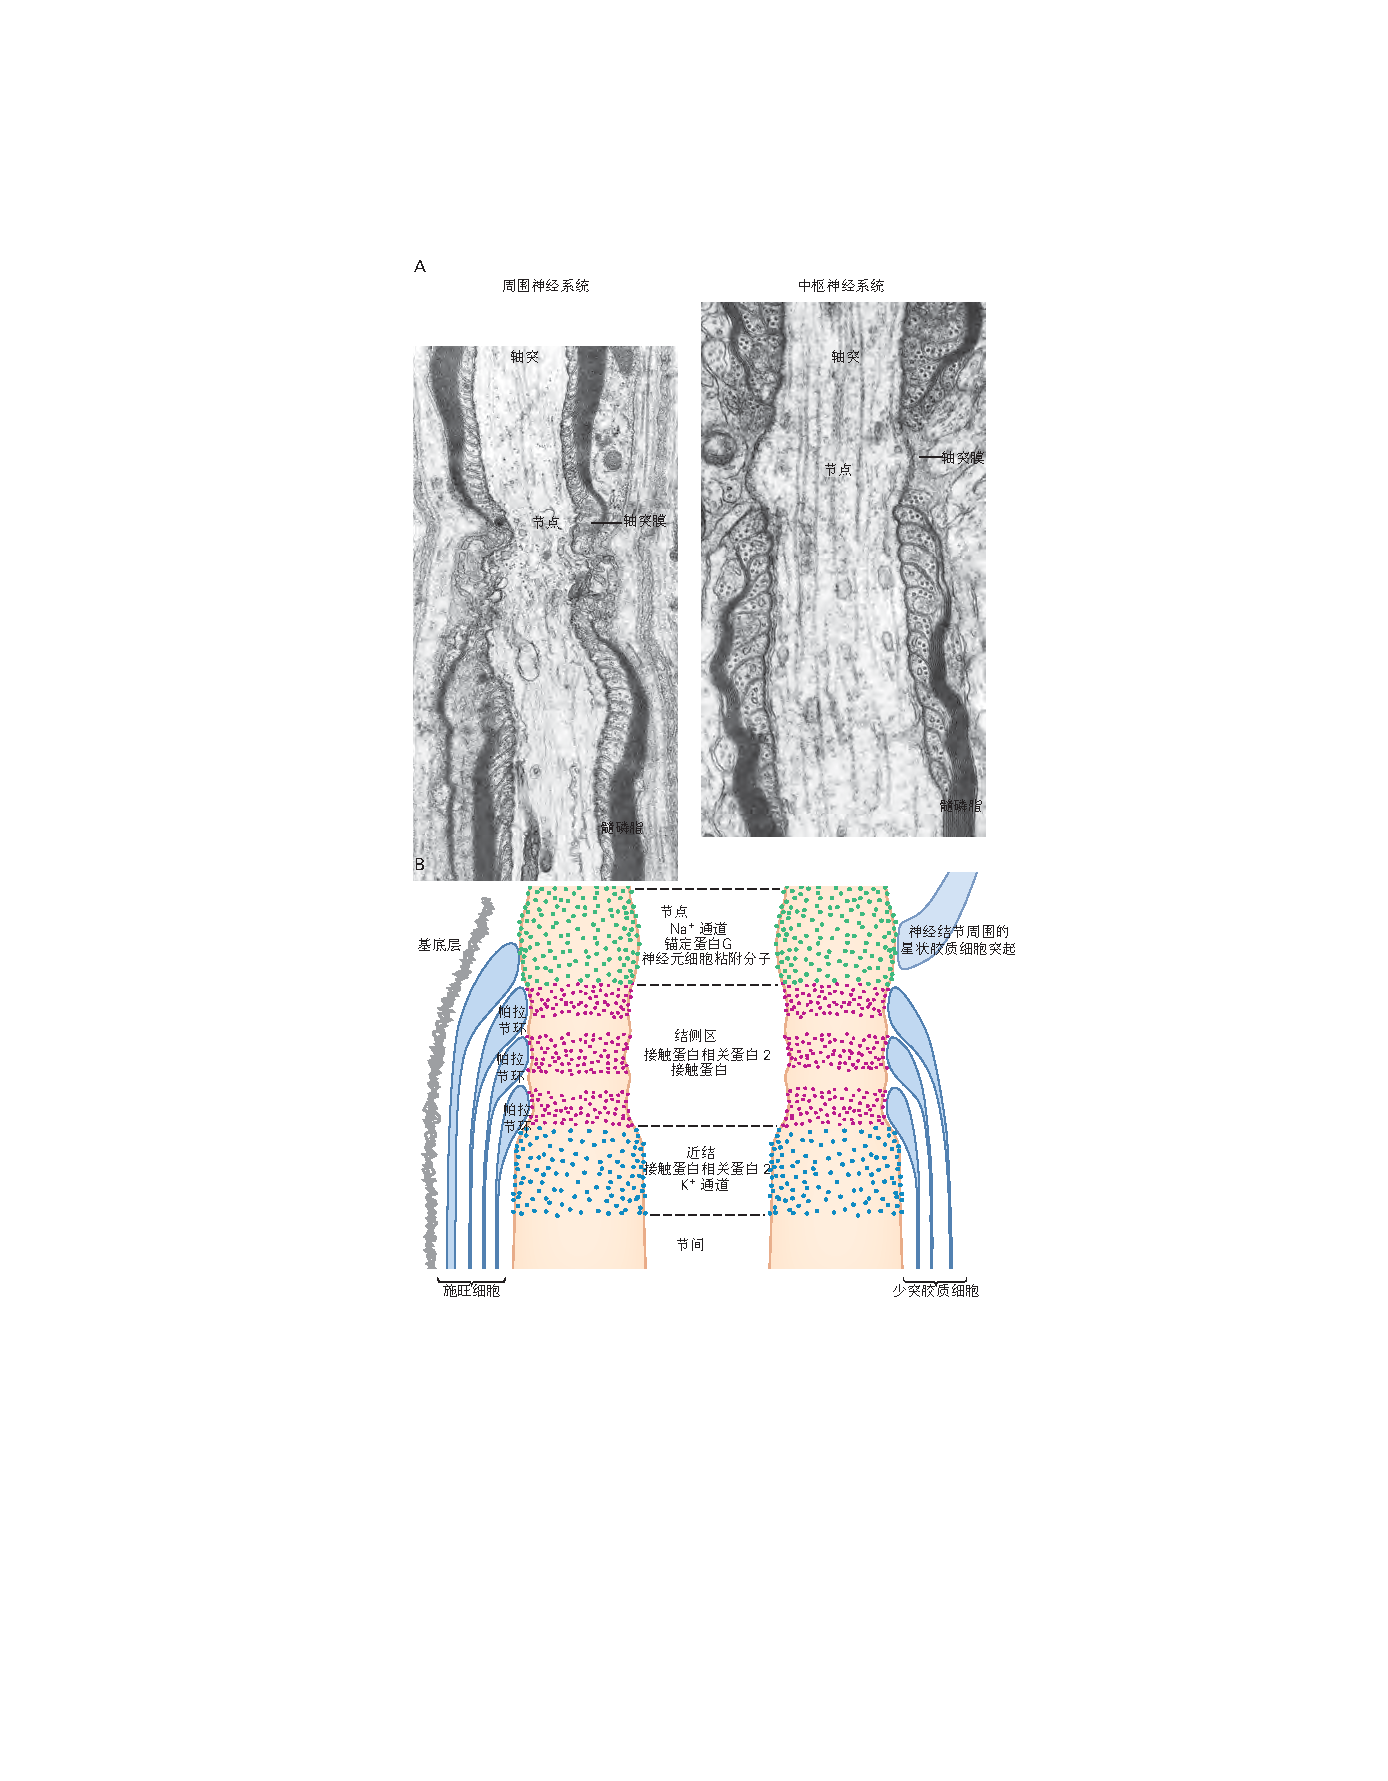
\includegraphics[width=0.75\linewidth]{chap07/fig_7_16}
	\caption{轴突的髓鞘有规则的间隙,称为郎飞结。
		A. 电子显微照片显示周围神经系统和脊髓轴突中的节点区域。
		\textit{轴突}在两张显微照片中都垂直延伸。
		\textit{髓磷脂}层在\textit{节点}处不存在,\textit{轴突膜}暴露在外\cite{peters1991neuropil}。
		B. \textit{郎飞结}两侧的区域富含髓鞘细胞和轴突之间的稳定接触,以确保节点不会移动或改变大小和限制轴突中 \ce{K+} 和~\ce{Na+} 通道的定位。
		\ce{K+}渗透通道和\textit{接触蛋白相关蛋白2}集中在\textit{近结}中。
		\textit{施旺细胞}或少突胶质细胞细胞质的\textit{帕拉节环}与轴突形成一系列稳定的连接。
		副节点区域富含粘附蛋白,如\textit{接触蛋白相关蛋白2}、接触素和\textit{神经束蛋白}155。
		在中央轴突的节点处,\textit{神经结节周围的星状胶质细胞突起}接触\textit{轴突膜},该膜上富含 \ce{Na+} 通道。
		\ce{Na+} 渗透性的这种定位是有髓轴突跳跃式传导的主要基础。
		膜细胞骨架连接物\textit{锚定蛋白G}、\textit{神经元细胞粘附分子}和\textit{神经束蛋白}186也集中在节点处\cite{peles2000molecular}。}
	\label{fig:7_16}
\end{figure}


在人类股神经中,初级感觉轴突长约0.5米,节间距离为1至1.5毫米;
因此,在大腿肌肉和背根神经节细胞体之间的初级传入纤维上大约有300至500个朗飞节。
因为每个节间节段由单个\textit{施旺细胞}形成,所以有多达 500 个\textit{施旺细胞}参与了每个外周感觉轴突的髓鞘形成。


髓鞘具有双分子脂质层,穿插在蛋白质层之间。
其成分与\textit{细胞质膜}相似,由 70\% 的脂质和 30\% 的蛋白质以及高浓度的胆固醇和磷脂组成。
在中枢神经系统中,髓磷脂有 2 种主要蛋白质:
髓磷脂碱性蛋白(一种小型的带正电荷的蛋白质)位于紧密髓鞘的细胞质表面,以及蛋白脂质蛋白(一种疏水性整体膜蛋白)。
这 2 种蛋白的功能可能是为鞘提供结构稳定性。



这 2 种蛋白也被认为是重要的自身抗原,免疫系统可以针对这些自身抗原产生反应,从而产生脱髓鞘疾病多发性硬化症。
在周围神经系统中,髓磷脂含有一种主要的蛋白质\textit{髓磷脂零蛋白},以及疏水性蛋白质\textit{外周鞘磷脂蛋白22}。
对这些蛋白质的自身免疫反应会产生脱髓鞘周围神经病,即\textit{古兰-巴雷综合症}。
髓鞘蛋白基因的突变也会导致外周和中央轴突发生多种脱髓鞘疾病(文本框~\ref{box:7_3})。
脱髓鞘电流从\textit{轴突膜}漏出,会减慢甚至停止轴突中动作电位的传导。
因此,脱髓鞘疾病对中枢和周围神经系统的神经元回路具有破坏性影响(第~\ref{chap:chap57}~章)。


\begin{proposition}[髓鞘蛋白缺陷破坏神经信号传导] \label{box:7_3}
	
	\quad \quad 因为在有髓鞘轴突中,神经冲动的正常传导取决于髓鞘的绝缘特性,有缺陷的髓鞘会导致运动功能和感觉功能的严重紊乱。
	
	\quad \quad 许多影响髓鞘的疾病(包括一些脱髓鞘疾病的动物模型)都有遗传基础。
	\textit{颤抖}突变小鼠有颤抖和频繁抽搐,往往英年早逝。
	在这些小鼠中,中枢神经系统中轴突的髓鞘形成严重不足,并且确实发生的髓鞘形成是异常的。
	
	\quad \quad 导致这种疾病的突变是位于小鼠 18 号染色体上的髓鞘碱性蛋白基因的 6 个外显子中的 5 个缺失。
	突变是隐性的;
	只有从父母双方遗传了缺陷基因,老鼠才会患上这种疾病。
	如图~\ref{fig:7_17}A~所示,继承 2 种缺陷基因的Shiverer小鼠的\textit{髓磷脂碱性蛋白}仅为正常小鼠的约10\%。
	
	\quad \quad 当将野生型基因注射到\textit{颤抖}突变体的受精卵中以拯救突变体时,得到的转基因小鼠表达野生型基因,但仅产生正常量的20\%的\textit{髓磷脂碱性蛋白}。
	然而,转基因小鼠的中枢神经元髓鞘形成得到了很大改善。
	如图~\ref{fig:7_17}B~所示,尽管转基因小鼠偶尔仍有震颤,但它们没有抽搐,寿命正常。
	
	\quad \quad 在中枢和外周神经系统中,髓鞘都含有一种称为\textit{髓磷脂相关糖蛋白}的蛋白质。
	\textit{髓磷脂相关糖蛋白}属于免疫球蛋白超家族,包括几种被认为参与细胞间识别的重要细胞表面蛋白,例如抗原的主要组织相容性复合体、T细胞表面抗原和\textit{神经细胞粘附分子}。
	
	\quad \quad 在外周神经系统中,在髓鞘产生的早期,施旺细胞表达\textit{髓磷脂相关糖蛋白},并最终成为成熟(致密)髓鞘的组成部分。
	它的早期表达、亚细胞定位以及与其他表面识别蛋白的结构相似性表明,它是一种对髓鞘形成过程的启动很重要的粘附分子。
	\textit{髓磷脂相关糖蛋白}的 2 种异构体是由单个基因通过选择性\textit{核糖核酸}剪接产生的。
	
	\quad 成熟的外周髓磷脂中的主要蛋白质(\textit{髓磷脂零蛋白})横跨施旺细胞的\textit{细胞质膜}。
	它有一个基本的细胞内结构域,和\textit{髓磷脂相关糖蛋白}一样,是免疫球蛋白超家族的成员。
	该蛋白的糖基化细胞外部分包含免疫球蛋白结构域,在髓鞘包裹过程中,通过与附着膜表面上的相同结构域相互作用,起到同源粘附蛋白的作用。
	\textit{髓磷脂零蛋白}功能被消除的基因工程小鼠运动协调性差,产生震颤,偶尔抽搐。
	
	\quad 对震颤小鼠突变体的观察导致了\textit{外周鞘磷脂蛋白22}的鉴定。
	这种\textit{施旺细胞}蛋白横跨膜 4 次,通常存在于致密的髓鞘中。
	\textit{外周鞘磷脂蛋白22}被突变体中的单个氨基酸改变。
	在人类身上也发现了一种类似的蛋白质,由17号染色体上的一个基因编码。
	
	\quad \quad 如图~\ref{fig:7_18}~所示,17号染色体上\textit{外周鞘磷脂蛋白22}基因的突变会产生几种遗传性外周神经病变,而该基因的复制会导致一种形式的\textit{腓骨肌萎缩症}。
	这种疾病是最常见的遗传性周围神经病变,其特征是进行性肌无力、周围神经传导大大减少以及脱髓鞘和髓鞘再形成周期。
	由于 2 个重复的基因都是活性的,这种疾病是\textit{外周鞘磷脂蛋白22}产生增加的结果(基因剂量增加了 2 到 3 倍)。
	\textit{施旺细胞}表达的许多基因突变可以产生遗传性周围神经病变。
	
	\quad \quad 在中枢神经系统中,髓鞘中超过一半的蛋白质是\textit{蛋白脂蛋白},它有 5 个跨膜结构域。
	蛋白质与脂蛋白的不同之处在于它们不溶于水。
	蛋白脂质仅可溶于有机溶剂,因为它们含有与整个蛋白脂质分子的氨基酸残基共价连接的长脂肪酸链。
	相反,脂蛋白是蛋白质与脂质的非共价复合物,通常作为血液中脂质部分的可溶性载体。
	
	\quad \quad \textit{蛋白脂蛋白}的许多突变在人类和其他哺乳动物中都是已知的,例如\textit{神经髓鞘形成不全鼠}。
	一个例子是\textit{佩梅病}(一种人类的异质性X连锁疾病)。
	几乎所有的\textit{蛋白脂蛋白}突变都发生在分子的跨膜结构域中。
	突变动物的\textit{蛋白脂蛋白}数量减少,髓鞘形成减少,少突胶质细胞变性和死亡。
	这些观察结果表明\textit{蛋白脂蛋白}参与了髓鞘的压紧。
	
\end{proposition}


\begin{figure}[htbp]
	\centering
	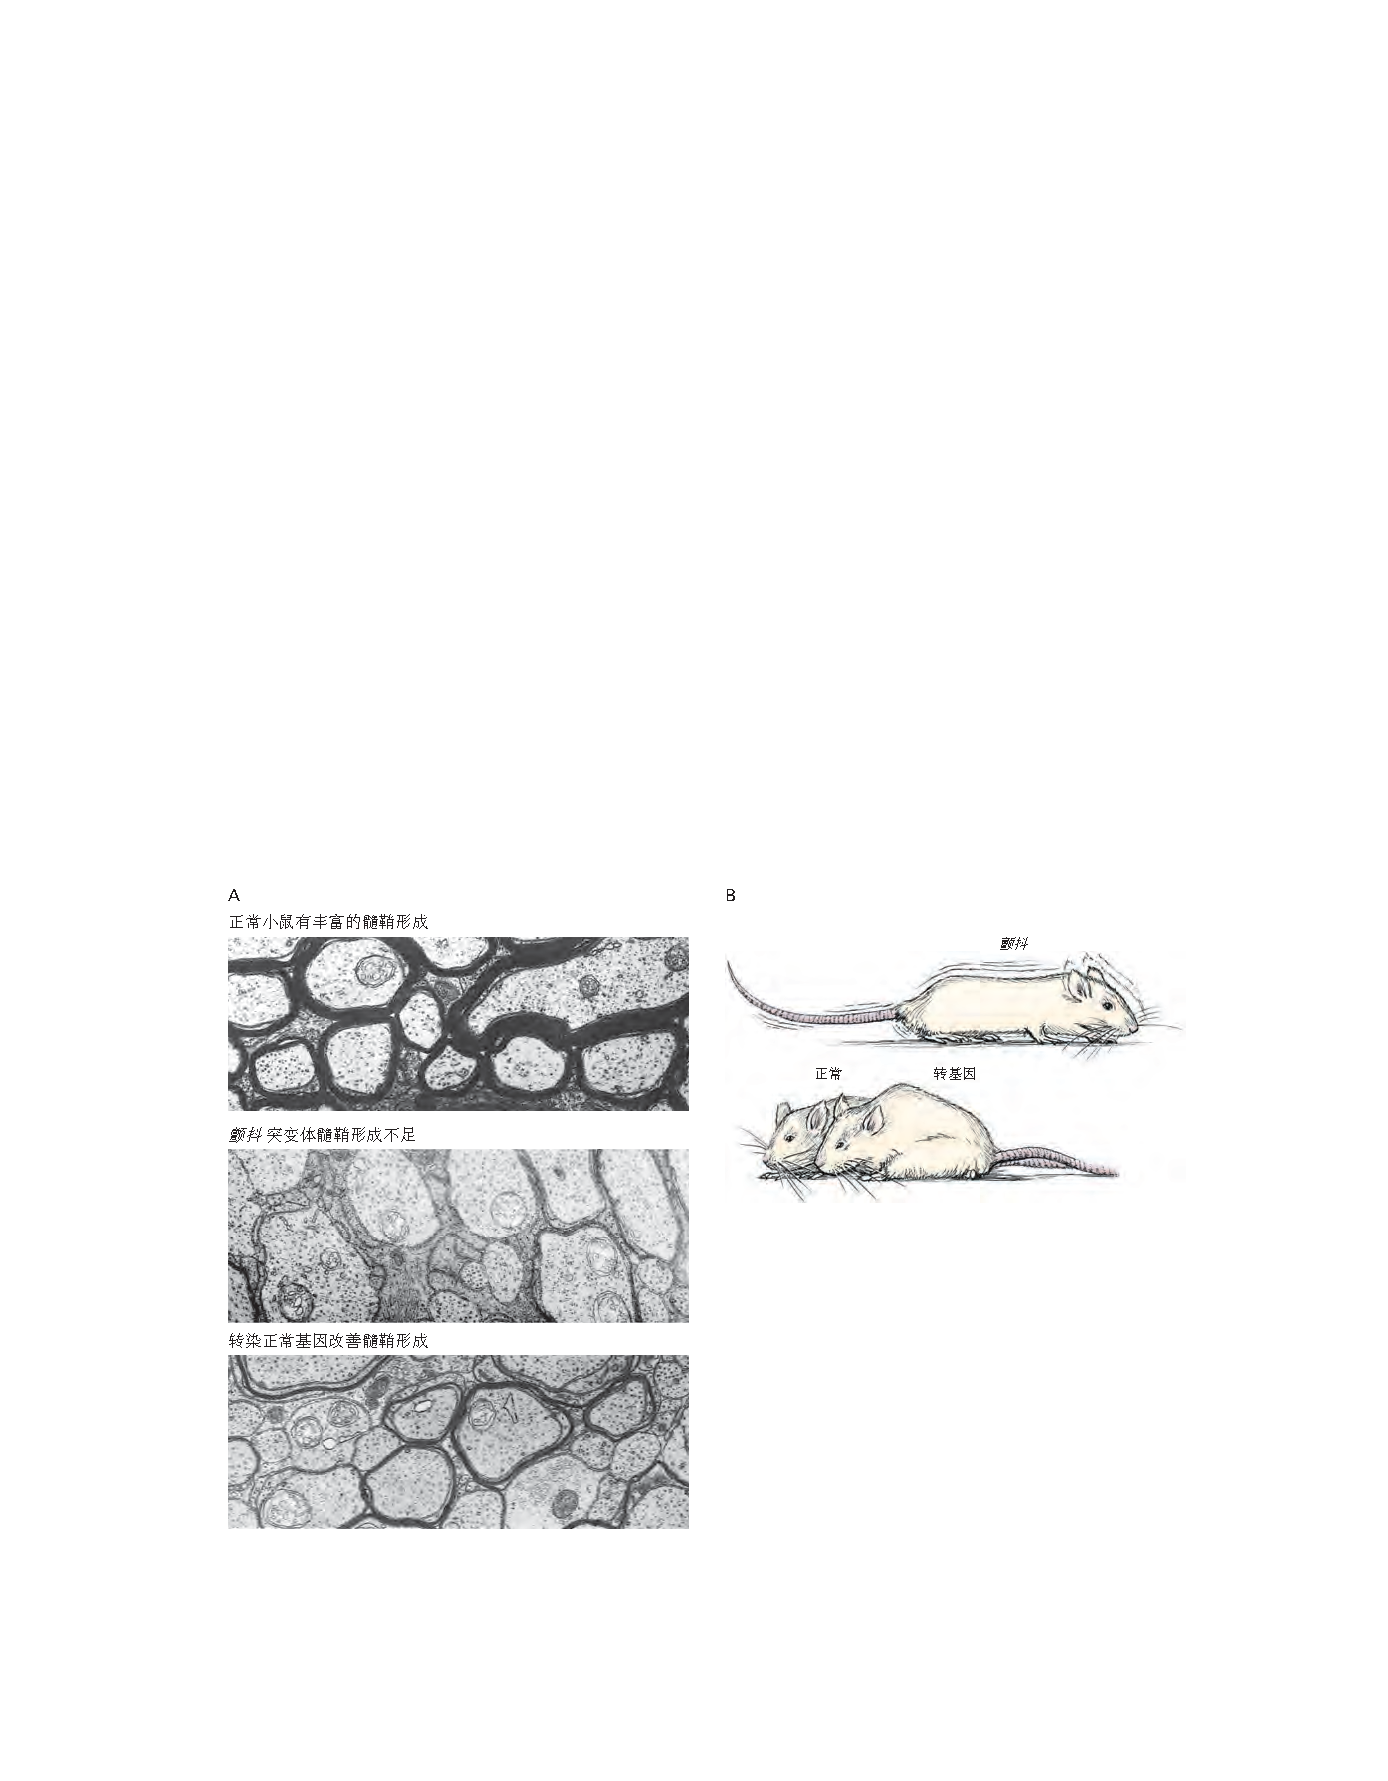
\includegraphics[width=1.0\linewidth]{chap07/fig_7_17}
	\caption{小鼠髓鞘形成的遗传性疾病可以通过转染编码髓鞘碱性蛋白的正常基因而部分治愈。
	A. 电子显微照片显示了一只正常小鼠、一只颤抖突变体和一只携带髓鞘碱性蛋白转染基因的颤抖突变体的视神经髓鞘形成状态。
	B. 颤抖突变体表现出不良的姿势和虚弱。
	将野生型基因注射到突变体的受精卵中改善髓鞘形成;
	经过处理的突变体看起来和正常小鼠一样活泼\cite{readhead1987expression}。}
	\label{fig:7_17}
\end{figure}


\begin{figure}[htbp]
	\centering
	\includegraphics[width=0.93\linewidth]{chap07/fig_7_18}
	\caption{\textit{腓骨肌萎缩症}(1A型)由外周髓磷脂蛋白22的产生增加引起。
	A. 一名患有\textit{腓骨肌萎缩症}的患者出现步态受损和畸形。}
	\label{fig:7_18}
\end{figure}




\subsection{\textit{星形胶质细胞}支持突触信号传递}

\textit{星形胶质细胞}存在于大脑的所有区域;
实际上,它们几乎占脑细胞数量的一半。
它们在滋养神经元和调节细胞外空间中离子和神经递质的浓度方面发挥着重要作用。
但是星形胶质细胞和神经元也可以相互交流以调节突触信号,其方式仍知之甚少。
星形胶质细胞通常分为两大类,它们在形态、位置和功能上各不相同。
原生质星形胶质细胞存在于灰质中,它们的活动与突触和血管密切相关。
白质中的纤维状星形胶质细胞与轴突和\textit{郎飞结}相接触。
此外,特殊的星形胶质细胞包括小脑中的\textit{贝格曼胶质细胞}和视网膜中的\textit{米勒胶质细胞}。


星形胶质细胞有大量细长的突触,它们包裹着大脑的所有血管,并包裹着突触或突触群。
如图~\ref{fig:7_19}~所示,星形胶质细胞与突触的密切物理联系非常紧密,它们之间的距离通常小于 1 微米,因此星形胶质细胞可以调节细胞外离子、神经递质和其他分子的浓度。
事实上,星形胶质细胞能够表达许多与神经元相同的电压门控离子通道和神经递质受体,因此它们能够很好地接收和传输可能影响神经元兴奋性和突触功能的信号。


\begin{figure}[htbp]
	\centering
	\includegraphics[width=1.0\linewidth]{chap07/fig_7_19}
	\caption{\textit{星状胶质细胞突起}与突触密切相关。
		A. 星形胶质细胞占据离散的体积。
		显示中心星形胶质细胞(绿色)占据的体积与其 3 个邻居(红色)不同,仅在其突起末端有少量重叠(黄色),这些突起通过\textit{细胞间隙连接}进行互联,图中比例尺条带长为 20 微米\cite{bushong2002protoplasmic}。
		B. 这张高压电子显微照片显示了几个粗突起从星形胶质细胞的细胞体发出,并分成非常细的突起。
		血管的典型包络显示在右下角\cite{hama1994three}。
		C. 星形胶质细胞的过程与突触前和突触后元素密切相关。
		1. 在这张海马细胞的电子显微照片中可以看出星形胶质细胞突起和突触之间的密切联系\cite{ventura1999three}。
		2. 从突触前神经元释放的谷氨酸不仅激活突触后神经元上的受体,还激活\textit{$\alpha$-氨基-3-羟基-5-甲基-4-异恶唑丙酸}受体。
		星形胶质细胞通过高亲和力转运蛋白摄取从突触间隙去除谷氨酸\cite{gallo2001unwrapping}。}
	\label{fig:7_19}
\end{figure}


星形胶质细胞如何调节轴突传导和突触活动?
首先是~\ce{K+} 的缓冲作用。
当神经元产生动作电位时,它们会将~\ce{K+} 释放到细胞外。
由于星形胶质细胞的膜上具有高浓度的~\ce{K+} 通道,因此它们可以充当空间缓冲器:
它们在神经元活动场所(主要是突触)吸收~\ce{K+},并在与血管的远距离接触处释放~\ce{K+}。
星形胶质细胞还可以在其细胞质过程中局部积聚~\ce{K+}、~\ce{Cl-}和水。
不幸的是,星形胶质细胞中离子和水的积聚会导致头部受伤后出现严重的脑肿胀。


星形胶质细胞还调节大脑中的神经递质浓度。
例如,如图~\ref{fig:7_19}C~所示,位于星形胶质细胞质膜中的高亲和力转运蛋白可快速清除突触间隙中的神经递质谷氨酸。
一旦进入神经胶质细胞,谷氨酸就会被谷氨酰胺合成酶转化为谷氨酰胺。
然后谷氨酰胺被转移到神经元,在那里它会作为生产谷氨酸的直接前体(第~\ref{chap:chap16}~章)。
若这些摄取机制受到干扰,则会导致细胞外谷氨酸浓度过高,从而导致神经元死亡,这一过程被称为兴奋性毒性。
星形胶质细胞还能够降解多巴胺、去甲肾上腺素、肾上腺素和\textit{5-羟色氨}。


% Astrocytes sense when neurons are active
星形胶质细胞会感知神经元何时活跃,因为它们会被神经元释放的~\ce{K+} 去极化,并且具有与神经元相似的神经递质受体。
例如,小脑中的\textit{贝格曼胶质细胞}就能够表达谷氨酸受体。
因此,小脑突触释放的谷氨酸不仅影响突触后神经元,还会影响突触附近的星形胶质细胞。
这些配体与神经胶质受体的结合增加了细胞内游离\ce{Ca^2+}浓度,从而会造成一些重要的影响。
一个星形胶质细胞的突起通过称为间隙连接的细胞间水通道与邻近星形胶质细胞的突起相连(第~\ref{chap:chap11}~章),从而实现离子和小分子在许多细胞之间进行转移。
一个星形胶质细胞内游离\ce{Ca^2+}浓度的增加会导致相邻星形胶质细胞中\ce{Ca^2+}的浓度的增加。
这种\ce{Ca^2+}在星形胶质细胞网络中的扩散可达数百微米范围。
这种\ce{Ca^2+}的扩散很可能通过触发营养物质的释放和调节血流来影响附近的神经元活动。
星形胶质细胞中\ce{Ca^2+}的增加会导致能够增强突触功能的信号的分泌。
因此,星形胶质细胞-神经元信号的传导有助于维持正常的神经回路功能。


星形胶质细胞对于突触的发育也很重要。
它们在产后大脑突触处的出现与突触发生和突触成熟的时期一致。
星形胶质细胞为突触形成准备神经元表面并稳定新形成的突触。
例如,星形胶质细胞分泌多种突触因子,包括血小板反应蛋白、\textit{高内皮静脉蛋白}和一种\textit{蛋白聚糖}glycipans,它们促进新突触的形成。
星形胶质细胞还可以通过吞噬作用帮助重塑和消除发育过程中多余的突触(第~\ref{chap:chap48}~章)。
在成人\textit{中枢神经系统}中,星形胶质细胞继续吞噬突触,并且由于这种吞噬作用依赖于神经元活动,因此突触的这种重塑可能有助于学习和记忆。
在病理状态下,例如轴突受损导致染色质溶解时,星形胶质细胞和突触前末端会暂时从受损的突触后细胞体中缩回。
星形胶质细胞释放神经营养因子和胶质营养因子,促进神经元和少突胶质细胞的发育和存活。
它们还保护其他细胞免受氧化应激的影响。
例如,星形胶质细胞中的谷胱甘肽过氧化物酶能对缺氧、炎症和神经元变性过程中释放的有毒氧自由基进行解毒。


最后一点,星形胶质细胞包裹着整个大脑中的小动脉和毛细血管,在星形胶质细胞突起的末端和内皮细胞周围的基底膜之间形成接触。
\textit{中枢神经系统}与全身血液循环隔绝,因此血液中的大分子不会被动进入大脑和脊髓(血脑屏障)。
血脑屏障主要是因内皮细胞和大脑毛细血管之间紧密连接产生的,身体其他部位的毛细血管并不具备这一特征。
然而,内皮细胞具有许多运输特性,允许一些分子通过它们进入神经系统。
由于星形胶质细胞和血管的密切接触,葡萄糖等被运输的分子可以被星形胶质细胞的末端吸收。


脑损伤和疾病发生后,星形胶质细胞会发生剧烈转变,被称为反应性星形胶质细胞增多症,其中涉及基因表达、形态和信号传导的变化。
反应性星形胶质细胞的功能十分复杂,人们对其了解甚少,因为它们既能阻碍中枢神经系统的恢复,也能支持中枢神经系统的恢复。
最近的研究发现,至少存在 2 种反应性星形胶质细胞;
一种有助于促进修复和恢复,而另一种则有害,会在中枢神经系统急性损伤后导致神经元的死亡;
不过,很可能还有其他亚型的反应性星形胶质细胞。
这些神经毒性反应性星形胶质细胞在阿尔茨海默病和其他神经退行性疾病患者中很突出,因此是一种有吸引力的新疗法靶点。
一个有趣的问题是:为什么大脑会产生神经毒性反应性星形胶质细胞。
很有可能是因为,移除受伤或患病的神经元可以使突触重组,从而有助于保持神经回路的功能。
此外,移除被病毒感染的神经元还有助于限制病毒感染的传播。


\subsection{小胶质细胞在健康和疾病中具有多种功能}

小胶质细胞约占中枢神经系统神经胶质细胞的 10\%,并以多种形态存在于健康和受损的大脑中。
尽管 100 多年前\textit{瑞鸥$\cdot$霍特加}就已经描述过小胶质细胞,但与其他细胞类型相比,人们对小胶质细胞的功能仍知之甚少。
与神经元、星形胶质细胞和少突胶质细胞不同,小胶质细胞不属于神经外胚层谱系。
长期以来,人们一直认为小胶质细胞来源于骨髓,但最近的命运图谱研究发现,小胶质细胞实际上来源于卵黄囊中的骨髓祖细胞。


如图~\ref{fig:7_20}~所示,小胶质细胞在胚胎发育的早期就在大脑聚集,并终存在在于大脑的各个区域。
如图~\ref{fig:7_21}~所示,在发育过程中,小胶质细胞通过吞噬突触前和突触后结构来帮助塑造发育中的神经回路,并且有新出现的证据表明,小胶质细胞可能在大脑发育和大脑稳态的其他方面也起着调节作用。
最近的体内成像研究揭示了小胶质细胞和神经元之间的动态相互作用。
在健康的成人大脑皮层中,小胶质细胞不断检测它们周围的细胞外环境并接触神经元和突触,但这种活动的功能意义仍然未知。


\begin{figure}[htbp]
	\centering
	\includegraphics[width=0.9\linewidth]{chap07/fig_7_20}
	\caption{大量的小胶质细胞存在于哺乳动物的中枢神经系统中。
		左边的显微照片显示了成年小鼠大脑皮层中的小胶质细胞(棕色,免疫细胞化学)。
		蓝色斑点是非微胶质细胞的细胞核。
		如右图所示,小胶质细胞有精细的花边状突起。}
	\label{fig:7_20}
\end{figure}


\begin{figure}[htbp]
	\centering
	\includegraphics[width=0.5\linewidth]{chap07/fig_7_21}
	\caption{在健康的大脑中,小胶质细胞与突触元件相互作用并塑造突触元件。
		成年小鼠嗅球中的双光子成像显示:表达\textit{分形趋化因子}受体-\textit{绿色荧光蛋白}融合物(绿色)的小胶质细胞突起连接到\textit{红色荧光蛋白}标记的神经元(红色)。}
	\label{fig:7_21}
\end{figure}


在受伤和疾病之后,小胶质细胞的运动过程会急剧增加,它们的形态和基因表达也会发生变化,并且可以迅速聚集到损伤部位,在那里它们可以发挥有益的作用。
例如,它们可以将淋巴细胞、中性粒细胞和单核细胞带入中枢神经系统并扩大淋巴细胞数量,这在感染、中风和免疫脱髓鞘疾病中是重要的免疫活动。
淋巴细胞还能吞噬碎屑、不需要的细胞和濒死细胞以及有毒蛋白质,从而保护大脑,这对于防止进一步损伤和维持大脑稳态至关重要。
虽然小胶质细胞对感染或创伤的免疫反应至关重要,但它们也会通过释放细胞因子和神经毒性蛋白以及诱导神经毒性反应性星形胶质细胞而导致病理性神经炎症。
在阿尔茨海默病和神经退行性疾病模型中,它们也会导致突触丢失和功能障碍。


\section{脉络丛和室管膜细胞产生脑脊液}

神经元和胶质细胞的功能受中枢神经系统细胞外环境的严格调控。
\textit{间质液}填充实质中神经元和胶质细胞之间的空间。
\textit{脑脊液}充满脑室、大脑和脊髓的蛛网膜下腔以及中枢神经系统的主要脑池。
\textit{间质液}和\textit{脑脊液}将营养物质输送到\textit{中枢神经系统}中的细胞,维持离子稳态,并作为代谢废物的清除系统。
\textit{脑脊液}与围绕大脑和脊髓的脑膜层一起提供保护\textit{中枢神经系统}组织免受机械损伤的缓冲层。
\textit{中枢神经系统}的液体环境由血脑屏障的内皮细胞和血脑脊液屏障的脉络丛上皮细胞维持。
这些屏障不仅用于调节大脑和脊髓的细胞外环境,而且还在中枢神经系统和外周之间传递关键信息。


脉络丛和室管膜层的细胞有助于\textit{脑脊液}的产生、组成和活动。
脉络丛在神经管闭合后不久表现为上皮内陷,最终将形成侧脑室、第三脑室和第四脑室。
经过胚胎发育,脉络丛逐渐成熟,每个脉络丛形成一个纤毛立方上皮层,包裹基质和免疫细胞网络以及广泛的毛细血管床。
室管膜是单层纤毛立方细胞(一种排列在脑室的神经胶质细胞)。
如图~\ref{fig:7_22}B~所示,在侧脑室和第四脑室的一些部位,特定的室管膜细胞形成了围绕脉络丛的上皮层。


\begin{figure}[htbp]
	\centering
	\includegraphics[width=1.0\linewidth]{chap07/fig_7_22}
	\caption{\textit{室管膜}和\textit{脉络丛}。
		A. 室管膜是排列在\textit{脑室}内的单层纤毛立方细胞。
		下图是室管膜衬里的高倍放大图(上图中为矩形),显示室管膜细胞心室侧的纤毛。
		B. 脉络丛与室管膜连续,但伸入心室,覆盖薄血管,形成分支非常多的乳头状结构。
		这是脑脊液形成的部位。
		高倍镜(下图)显示\textit{血管}核心和上覆的\textit{脉络丛}。
		箭头表示在脑脊液形成过程中,流体从毛细管流入心室的方向。}
	\label{fig:7_22}
\end{figure}


脉络丛产生大部分沐浴大脑的脑脊液。
室管膜细胞之间的松散连接为脑脊液提供了进入大脑间质空间的通道。
如图~\ref{fig:7_22}A~所示,室管膜细胞中的纤毛运动有助于脑脊液穿过心室系统,促进分子向中枢神经系统中的其他细胞进行远距离输送,并将废物从中枢神经系统输送到外周。


脉络丛将液体和溶质从血清输送到中枢神经系统以产生脑脊液。
穿过脉络丛的有孔毛细血管允许水和小分子从血液中自由通过进入脉络丛的基质空间。
然而,脉络丛上皮细胞会形成紧密连接,防止这些分子进一步不受控制地进入大脑。
相反,组成\textit{脑脊液}的水、离子、代谢物和蛋白质介质的输入受到脉络丛上皮中转运蛋白和通道的严格调控。
上皮细胞中的主动运输机制是双向的,另外还介导分子从\textit{脑脊液}返回外周循环的流量。


脉络丛上皮细胞也能够合成许多蛋白质并将其分泌到脑脊液中。
在健康的胚胎和出生后的大脑中,这些蛋白质调节神经干细胞的发育,并可能调节皮层可塑性等过程。
脉络丛上皮细胞分泌蛋白组也可以因来自外周或大脑内部的炎症信号而发生改变,从而对感染和衰老过程中的神经元的功能产生影响。
其他脉络丛衍生因子在健康和患病大脑中的功能作用(包括\textit{微小核糖核酸}、长链非编码\textit{核糖核酸}和细胞外囊泡)也开始显现出来,进一步强调了这种结构对大脑发育和\textit{内稳态}的重要贡献。



\section{亮点}

1. 神经元的形态非常适合在大脑中接收、传导和传递信息。
树突为接收信号提供了高度分支的细长表面。
轴突长距离快速传导电脉冲到它们的\textit{突触末稍},\textit{突触末稍}将神经递质释放到目标细胞上。


2. 尽管所有神经元都符合相同的基本细胞结构,但不同亚型的神经元在其特定的形态特征、功能特性和分子特性方面差异很大。


3. 不同位置的神经元在其树突树的复杂性、轴突分支的范围以及它们形成和接收的\textit{突触末稍}数量方面存在差异。
这些形态差异的功能意义显而易见。
例如,运动神经元必须具有比感觉神经元更复杂的树突树,因为即使是简单的反射活动也需要整合许多兴奋性输入和抑制性输入。
不同类型的神经元使用不同的神经递质、离子通道和神经递质受体。
这些生物化学、形态学和电生理学的差异共同导致了大脑中信息处理的巨大复杂性。


4. 神经元是我们体内极化程度最高的细胞之一。
它们的树突和轴突区室的巨大尺寸和复杂性代表了这些细胞面临的重大细胞生物学挑战,包括长距离运输各种细胞器、蛋白质和\textit{信使核糖核酸}(某些轴突可达 1 米)。
大多数神经元蛋白在细胞体内合成,但一些合成发生在树突和轴突中。
新合成的蛋白质在\textit{伴侣蛋白}的帮助下进行折叠,其最终结构通常通过永久性或可逆的翻译后修饰进行改变。
神经元中蛋白质的最终目的地取决于其氨基酸序列中编码的信号。


5. 蛋白质和\textit{信使核糖核酸}的转运具有很强的特异性,这些特异性导致了选定膜成分的分子转运。
细胞骨架除了控制轴突和树突形态外,还为将细胞器运输到不同的细胞内位置提供了重要的框架。


6. 所有这些基本的细胞生物学过程都可以通过神经元活动进行深刻的修改,从而使神经回路适应经验(学习)的细胞结构和功能发生巨大变化。


7. 神经系统还包含几种类型的神经胶质细胞。
少突胶质细胞和\textit{施旺细胞}产生髓鞘绝缘层,使轴突能够快速传导电信号。
星形胶质细胞和非髓鞘化\textit{施旺细胞}包裹着神经元的其他部分,尤其是突触。 
星形胶质细胞控制细胞外离子和神经递质浓度,并积极参与突触的形成和功能。
小胶质细胞常驻的免疫细胞和吞噬细胞与神经元和神经胶质细胞动态相互作用,并在健康和疾病中发挥多种作用。


8. 脉络丛和室管膜层的细胞有助于\textit{脑脊液}的产生、组成和活动。


9. 基因组学和单细胞\textit{核糖核酸}测序的新进展开始定义细胞类型的巨大多样性,不仅在神经元之间而且在神经胶质细胞之间。


10. 遗传学、细胞生物学和体内显微术(双光子显微术、光片显微术)的最新进展为神经元在整个生命周期中建立和维持其极性的独特机制提供了新的见解。


11. 这些新见解为细胞生物学步骤提供了重要线索,例如轴突运输缺陷,这些缺陷会引发亨廷顿病、帕金森病和阿尔茨海默病等神经退行性疾病。



